\documentclass[12pt, a4paper]{article}
\usepackage[utf8]{inputenc} % если ваш файл содержит русский текст, нужно указать кодировку
\usepackage[T2A]{fontenc}
\usepackage[russian]{babel} % для того, чтобы писать русский текст
\usepackage{amsmath} % для команды equation*
\usepackage{hyperref} % для вставки ссылок
\usepackage{graphicx}
\usepackage[russian]{babel}
\parindent 0pt
\parskip 0pt
\usepackage{amsmath}
\usepackage{amssymb}
\usepackage{array}
\usepackage[left=2.3cm, right=3.3cm, top=1.7cm, bottom=1.7cm, bindingoffset=0cm]{geometry}
\usepackage{hyperref}
\usepackage{graphicx}
\usepackage{float}
\usepackage{enumitem}
\usepackage{array}
\usepackage{subcaption}
\usepackage{multicol}
\usepackage{fancyhdr} 
\usepackage{extramarks}
\usepackage{todonotes}
\usepackage{color}
\graphicspath{{pictures/}}
\usepackage{lipsum}                     % Dummytext
\usepackage{xargs}                      % Use more than one optional parameter in a new commands
\usepackage{xcolor}

\usepackage{setspace}
\onehalfspacing

\title{Математический анализ.}
\author{Автор конспекта: Терентьев Михаил, Константин Ништ}
\date{\today}

\pagestyle{fancy}
\fancyhf{}
\lhead{Билет № 100500}
\chead{Математический анализ}
\rhead{\thepage}
\lfoot{Автор конспекта: Терентьев Михаил }
\cfoot{}
\rfoot{\today}
\renewcommand\headrulewidth{0.4pt}
\renewcommand\footrulewidth{0.4pt}
\newcommand{\nl}{\newline}
\newcommand{\intba}{\int^b_a}

\newcommand{\insertref}[1]{\todo[color=green!40]{#1}}
\newcommand{\explainindetail}[1]{\todo[color=red!40]{#1}}

\newcommand{\proof}{\textbf{\underline{Доказательство:}} }
\newcommand{\then}{\textbf{Тогда:}}

\setenumerate{topsep=0ex,itemsep=0ex,partopsep=0ex,parsep=0ex}

\begin{document}
	\section{TODO TUTORIAL}
	
	\todo{Make a cake \ldots}
	Look, this is TODO\insertref{actually what to change};
	
	\section{Правила оформления конспекта}
	\begin{enumerate}
		\item Используйте \verb|\leqslant|($\leqslant$) и \verb|\geqslant|($\geqslant$)
		\item После интегралов и сумм используйте \verb|\limits| для границ \nl
		С \verb|\limits| : $\int \limits^b_a, \;\;\; \sum \limits_{i = 1}^{\infty}$ \nl
		Без : $\int^b_a,\;\;\; \sum_{i = 1}^{\infty}$
		\item Не забывайте про \verb|\;| или \verb|\thickspace| между формулами, после запятых
		\item Теги \verb|\then| - \then, \verb|\proof| - \proof  
		\item Для списков используйте \verb|\begin{enumerate}| или \verb|\begin{itemize}| 
		\item Очень помогает latex cheatsheet - гуглите
	\end{enumerate}
	
	\newpage
	\section{Неопределённый интеграл}
	\lfoot{Автор конспекта: Константин Ништ}
	\subsection{Определение 1}
	$ f : <a; b> \rightarrow \mathbb{R} \newline
	\text{Тогда } F : <a; b> \rightarrow \mathbb{R} 
	\text{ называется первообазной (для f на }<a; b>),
	\text{если } \forall x \in <a; b> F'(x) = f(x)
	$
	
	\subsection{Определение 2}
	$ f : <a; b> \rightarrow \mathbb{R} \newline 
	\text{Неопределенный интеграл } \int f  
	\text{ - множество всех первообразных } F \text{ от } f \newline
	\int f = F + c, \text{ где } с \text{ - любая константа}
	$
	
	\subsection{Теорема 1}
	$f \text{ непрерывна } \Rightarrow \exists F \newline$
	\text{Потом докажут}
	
	\subsection{Теорема 2}
	Пусть F первообразная для $f$ на $<a; b> \\ $
	\then
	\begin{enumerate}
		\item $\forall c \in \mathbb{R}$ : F + C — первообразная 
		\item Других первообразных не существует : Если  G первообразная для f, то $\exists C_1 : F = G + C_1$
	\end{enumerate}
	\proof
	\begin{enumerate}
		\item Очевидно, что (F+C)' = F' + C' = F' + 0 = F' 
		\item (G(x)-F(x))' = f(x) - f(x) = 0. Тогда G-F = const.
	\end{enumerate}
	
	\subsection{Теорема о свойствах неопределённого интеграла}
	Пусть f и g имеют первообразную на <a; b>, $\alpha , \beta \in \mathbb{R} \newline$
	\then
	\begin{enumerate}
		\item $\int f + g = \int f + \int g $
		\item $\int \alpha f = \alpha  \int f $
		\item $\varphi : <c; d> \rightarrow <a; b>$ дифф 
		$\int f(\varphi(t)) \varphi ' (t)dt = \int f(x)dx | x = \varphi(t) $
		\item $\int f(\alpha x + \beta)dx = \frac{1}{\alpha} F (\alpha x + \beta) + C$
		\item f и g дифференцируемы на <a; b> f'g имеет первообразную. Тогда : \\
		fg' имеет первообразную и $\int fg' = fg - \int f'g $
	\end{enumerate}
	\proof
	\begin{enumerate}
		\item $(F + G)' = f + g $
		\item $(\alpha F)'$ = $\alpha f $
		\item[3-4.] Аналогично по свойсту диффа композиции 
		\item[5.] (fg)' = f'g + fg'; fg' = (fg)' - f'g 
		$(fg- \int f'g)' = (fg' - f'g) = fg'$
	\end{enumerate}
	
	\section{Равномерная непрерывность}
	\subsection{Определение}
	f : <a; b> $\rightarrow \mathbb{R}$ называется равномерно непрерывной на <a;b>, если : \nl
	$\forall \epsilon >0 \thickspace \exists \delta > 0 \thickspace \forall x, \thickspace x' \in <a;b>, \thickspace |x-x'|<\delta : f(x)-f(x')<\epsilon \nl$
	Примеры :
	\begin{enumerate}
		\item $f(x) = x, <a; b> = \mathbb{R}$ равномерно непрерывна 
		\item $f(x) = x^2$ не равномерно непрерывна 
	\end{enumerate}
	
	
	\subsection{Теорема Кантора о равномерной непрерывности} 
	$f : X \rightarrow Y$ непрерывно на Х, Х компактно. \nl
	Тогда $f$ равномерно непрерывна \nl
	Доказательство(от противного):
	$$ \exists \epsilon \forall \delta = \frac{1}{n} \exists x_n, {x'}_n \varrho(x_n, {x'}_n) < \delta $$
	$$ \rho(f(x_n),f({x'}_n)) \geqslant \epsilon $$ 
	Образовалась последовательность $x_n$ 
	$$\exists {x_n}_k \rightarrow a \in X $$ 
	$$ \rho({x_n}_k, {{x'}_n}_k)<\frac{1}{{n_k}} \Rightarrow {x_n}_k \rightarrow a $$ 
	$$ \rho(f({x_n}_k), f({{x'}_n}_k)) \geqslant \epsilon $$ 
	Но обе последовательности стремятся к $f(a)$, получено противоречие. \nl
	Следствие: $f : [a; b] \rightarrow \mathbb{R}$ непрерывно, тогда f равномерно непрерывно (например, $\sqrt{x}$);
	
	\section{Теорема Брауэра о неподвижной точке (БЕГИ И НЕ ОГЛЯДЫВАЙСЯ)}
	\subsubsection{Игра в гекс}
	Вдруг кто-то захочет упороться : \url{https://arxiv.org/pdf/1409.7890v1.pdf} \nl
	Представим себе ромбовидное поле n на m, состоящее из шестиугольников. Каждый игрок (чёрный и белый) владеет парой противоположных сторон ромба. За каждый ход игрок раскрашивает один из шестугольников. \nl
	Лемма : Любая раскраска игровой доски определяет выигрыш кого-то из игроков. \nl
	Рассмотрим левый край ромба. Выберем ребро на карте, которое разделяет чёрную и белую клетки (причём выберем ребро принадлежащее левому краю и ближайшее к нижнему левому углу). Будем идти по вершинам карты, причём каждый раз будем выбирать именно ту вершину, ребро до которой разделяет чёрную и белую клетки. Таким образом, всегда выполняется инвариант для игры : по "левую руку" от нас находится клетка одного цвета, по "правую" противоположного. Утверждается, что зациклиться мы не можем, ибо каждая вершина принадлежит трём клеткам, и если мы пошли по одному ребру и вернулись в ту же вершину, то одна и та же вершина окажется двух противоположных цветов (что, конечно же, звучит как бред). Таким образом мы сможем дойти до конца, и, так как наш путь содержит начало пути двух цветов, мы сможем точно определить победителя. Лемма доказана. \nl
	
	\subsection{Теорема Брауэра}
	$f : [0; 1]^n \in \mathbb{R}^n \rightarrow [0; 1]^n, \; f $ непрерывна. \nl
	\then
	$$\exists x \in [0; 1]^n : f(x) = x$$
	\proof (при n=2) 
	$$ x, y \in [0; 1] $$
	$$ x = (x_1, x_2); y = (y_1, y_2); \; \rho(x,y) = max(|x_1-y_1|, |x_2-y_2|) $$
	Пусть $ \forall x f(x) != x$ \nl
	По теорееме Виерштрасса существует такой минимум, что: 
	$$ \forall x \rho(x, f(x))>0 ; \;\; 0 < \epsilon = min(\rho(x, f(x)))$$
	$f$ равномерно-непрерывна, значит 
	$$ \exists \delta > 0 : \forall x,y ||x-y|| < \delta ||f(x)-f(y)|| < \epsilon.$$ 
	Можно считать, что $\epsilon > \delta \nl$
	$ \exists n : \frac{1}{n} < \delta; Hex(n , n)$ — логическая доска.
	$v = (v_1, v_2) \rightarrow (\frac{v_1}{n}, \frac{v_2}{n}) \in [0; 1]$ вершина доски. \nl
	$color(v) = min(i \in \{1, 2\} : (f(\frac{v_i}{n})-\frac{v_i}{n})) \nl$ 
	Доска покрашена. \nl
	Рассмотрим одноцветный путь(существует по леммe) $v^0, v^1, \ldots , v^n$ 
	$$v^0_1 = 0; f_1(\frac{v^0_1}{n}-\frac{v^0_1}{n}) \geqslant\epsilon$$ 
	$$v^n_1 = 1; f_1(\frac{v^n_1}{n}-\frac{v^n_1}{n}) \leqslant-\epsilon$$ 
	Рассмотрим расстояние между соседними вершинами 
	$$ \rho(\frac{v^i}{n}, \frac{v^{i+1}}{n}) \leqslant \frac{\sqrt{2}}{n} < \delta < \epsilon $$
	Следовательно, мы не могли перескочить через $2 \cdot \epsilon$, то есть наше начальное утверждение неверно. \nl
	\textbf{Теорема доказана.}
	
	\section{Определённый интеграл}
	\subsection{Площадь}
	\subsubsection{Определение площади}
	E — совокупность всех окраниченных подмножеств в $\mathbb{R}^2$ \nl
	Площадь : $\delta : E \rightarrow [0; +\infty]$, причём :
	\begin{enumerate}
		\item Аддитивность : $A = A_1 \bigsqcup A_2 \Rightarrow \delta A = \delta A_1 + \delta A_2$
		\item Нормировка : $\delta([a; b] \times [c; d]) = (b-a) \cdot (d-c) \nl$
		Замечание : $\delta \text{ монотонна} : A \in B \Rightarrow \delta A \leqslant \delta B$
	\end{enumerate}
	
	\subsubsection{Определение ослабленной площади}
	\begin{enumerate}
		\item Монотонна.
		\item Нормированна.
		\item Ослабленная аддитивность : $E = E_1 \bigcup E_2, E_1 \bigcap E_2$ вертикальный отрезок.
	\end{enumerate}
	\then $\;\; \delta E = \delta E_1 + \delta E_2$
	
	
	\subsection{Определённый интеграл}
	\subsubsection{Срезки}
	
	$f : <a; b> \rightarrow \mathbb{R} \nl$
	$f^+(x) = max(f(x), 0)$ положительная срезка. \nl
	$f^-(x) = min(f(x), 0)$ отрицательная срезка. \nl
	
	\subsection{Подграфик}
	Подграфиком функции $f$ на $[a; b] (f : [a;b]\rightarrow \mathbb{R}; f \geqslant 0)$ называют \nl
	ПГ(f([a;b])) = {$(x, y) \in \mathbb{R}^2, x \in [a; b], y \in [0; f(x)]$}
	
	\subsection{Определение интеграла}
	Определённым интегралом непрерывной функции $f$ по промежутку $[a;b]$ называется 
	$$ \int\limits^b_a f = \int\limits^b_a f(x) dx = \int\limits_{[a; b]} f(x) dx = \delta \text{ПГ}(f^+([a; b])) - \delta \text{ПГ}(f^-([a; b])) $$
	Замечание : $f \geq 0 \Rightarrow \int\limits^b_a \geq 0; \int\limits^a_a = 0$
	
	\subsection{Свойства интеграла}
	\subsubsection{Аддитивность по промежутку}
	$c \in [a;b]; f$ непрерывна на [a; b] \nl
	$\int_a^b f = \int_a^c f + \int^b_c f$ 
	
	\subsubsection{Монотонность} 
	$f, g \in C[a; b]; f \leqslant g \nl$
	Тогда $\int^b_a f \leqslant \int^b_a g$-интегрирование неравенств 
	
	\subsubsection{Теорема о среднем}l
	$f \in C[a;b]; \exists c \in [a;b] : \int^b_a f(x)dx = f(c) \cdot (b-a) \nl$
	Доказательство : \nl
	По теореме Вейерштрасса $min(f) \leqslant \frac{1}{b-a}\intba f \leqslant max(f) \nl$
	По теореме о промежуточном значении $\exists c : f(c) = \intba f$
	
	\subsubsection{Теорема Барроу}
	Определение: \nl
	$\Phi : [a;b] \rightarrow \mathbb{R}, f \in [a;b] \nl$
	$\Phi(x) = \int_a^x f$ интеграл с переменным верхним пределом. \nl
	$\Phi(a) = 0$
	Теорема : 
	$\Phi(x)$ дифф на [a; b] и $\forall x \in [a; b] \Phi'(x) = f(x)$ \nl
	Доказательство : \nl
	$x \in (a; b) \nl$
	y>x; $\lim_{y \to x+0} \frac{\Phi(y)-\Phi(x)}{y-x} = \lim_{y \to x+0}\frac{\int^y_x}{y-x} = \lim_{y \to x+0} f(c) = f(x) \nl $
	Также доказывается и левосторонняя производная. \nl
	Следствие : у любой непрерывной функции есть первообразная
	
	\subsubsection{Формула Ньютона-Лейбница}
	$f \in C[a; b]; F$ первообразная f на [a; b]\nl
	Тогда $\intba f(x)dx = F(b)-F(a) \nl$
	Доказательство : \nl
	$\Phi$ тоже первообразная. F = $\Phi + C\nl$
	$\intba f = \Phi(b)-\Phi(A) = F(b)-F(a)$
	
	
	
	
	
	\section{Выпуклость}
	\lfoot{Автор конспекта: Терентьев Михаил}
	%\begin{figure}[h!]
	%  \includegraphics[width=\linewidth]{ram-read.png}
	%  \caption{Чтение из памяти.}
	%  \label{fig:ram-read}
	%\end{figure}
	
	\subsection{Определение}
	A $\subset \mathbb{R}^m$ A - выпуклое множество \\
	$\forall x, y \in A$  $[x,y] \subset$ A \\
	$[x,y]=\lbrace x+t(y-x), t \in [0,1] \rbrace$ \\
	
	\subsection{Определение}
	f:<a,b> $\rightarrow \mathbb{R}$ - выпуклая функция \\
	$\forall \alpha \in [0,1] f (\alpha + (1-\alpha)y)< \alpha f(x) + (1-\alpha)f(y)$ \\
	
	\subsection{Лемма о трех хордах}
	1. f-выпуклая на <a,b> \\
	2. Если $x_{1} < x_{2} < x_{3}$  точки промежутка <a,b> \\
	$ \frac{f(x_2)-f(x_1)}{x_2-x_1}\leq\frac{\displaystyle f(x_3)-f(x_1)}{\displaystyle x_3-x_1}\leq\frac{\displaystyle f(x_3)-f(x_2)}{\displaystyle x_3-x_2}$ \\
	$(1) \leqslant> (2) (f(x_2-f(x_1))(x_3 -x_1) \leq (f(x_3)-f(x_{1}))(x_{2}-x_{1})$ \\
	
	\textbf{Док-во}
	
	$(f(x_3\frac{x_2-x_1}{x_3-x_1}+x_1\frac{x_3-x_2}{x_3-x_1})\;=\;f(x_2)\;)\;\leq\;f(x_3)\frac{x_2-x_1}{x_3-x_1}+f(x_1)\frac{x_3-x_2}{x_3-x_1}$
	
	\textbf{Замечание.} 
	f строго выпуклая <=> в неравенстве (2) знаки строгие \\
	\textbf{Наблюдение} f - выпуклая <=> f вогнутая \\
	f, g -выпуклая => f+g выпуклая 
	
	\subsection{Теорема об односторонней дифференцируемости вып функции}
	
	f- выпуклая на <a,b>. Тогда $\forall x \in <a,b> \exists f_{+}'(x) , f_{-}'(x)$ \\
	и $\forall x_{1}, x_{2} \in <a,b> x_{1}<x_{2}$ \\
	$f_{-}'(x_{1}) \leq f_{+}'(x_{1}) \leq \frac{f(x_2)-f(x_1)}{x_2-x_1}\leq f'(x_2)$ \\
	\textbf{Док-во} \\
	$g(\xi)=\frac{f(\xi)-f(x)}{\xi-x}$ \\ возр на <a,x> и на <x,b>  по лемме о трех хордах \\
	при $a\leq\xi_{1} < x<\xi_{2} < b $\\
	$ f_{+}'(x_{1})=l\lim_{\xi -> x_{1}+0}g(\xi) $\\
	$g(\xi)$ - монотонна, ограничена снизу  $\forall$ числом $g(\xi)$ таким , что$ \xi_0<x$ \\
	\textbf{Замечание} \\
	$ \text{На [a,b] возможна ситуация}  f_{+}'(a)= -\infty, f_{-}'(b)=+\infty$ \\
	$ \frac{f(x_2)-f(x_1)}{x_2-x_1} =g(\xi) \rightarrow $ (возр $ \xi -> x_{2}) f_{-}'(x_{2}) , x=x_{2}, \xi=x_{1} $\\
	$x=x_1, \xi=x_2 ; g(\xi) ->(\xi -> x_1 + 0) f_-(x_1)$ \nl
	
	$g(\xi_{1}) \leq g(\xi_{2})$ при $\xi_{2} \rightarrow x_1 + 0$ \\
	=> $g(\xi_{1}) \leq f_{+}'(x_{1})$ при $\xi_1 \rightarrow x_1 - 0$ \\
	=> $f_{-}'(x_1)  \leq f_{+}(x_{1})$  \\
	
	\subsection{Следствие} 
	f выпукла на <a,b> => f -непрерывен на <a,b> \nl
	$\exists$ кон  $f_{+}'(x)$ => f непр в т. x справа \nl
	$\exists$ кон  $f_{-}'(x)$ => f непр в т. x слева \nl
	
	\subsection{Теорема о выпуклостях в терминах касательных}
	f - дифф на $<a,b>$ 	\\
	Тогда f - вып вниз <=> График  f расположен не ниже касатльной \\
	$\forall x_{0},x f(x) \geq f(x_{0}) +f'(x_{0})(x-x_{0})$ \nl
	
	\textbf{Доказательство} \\
	=> Это неравенство содержится в предыдущей теореме \\
	<= $x_{1}< x_{0} < x_{2}$ \\
	$ f(x_{1})\geq f(x_{0})+f'(x_{0})(x_{1}-x_{0}) (1)$ \\
	$f(x_{2})\geq f(x_{0})+f'(x_{0})(x_{2}-x_{0}) (2)$ \\
	$\frac{f(x_2)-f(x_1)}{x_2-x_1} <f'(x_0)<\frac{f(x_2)-f(x_0)}{x_2-x_0}$ \text{ -- одно из н-в о 3-x хордах экв определению выпуклости}  \\
	
	
	l- проходит через точку $A \in E$, E расположено в одной полуплоскости относительно l ,\\
	l опорная прямая множества Е в т. А\\
	Для линии $y=f(x_0)+f_-'(x_0)(x-x_0)$ , при $x<x_0$ график лежит ниже  \\
	Для линии $y=f(x_0)+f_+'(x_0)(x-x_0)$ , при $x<x_0$ график лежит не ниже \\
	$min\lbrace y:(x,y)\in E \lbrace =: f(x_0) $-вып \textbf{здесь че-то не то в этой строчке} \\
	\subsection{о дифф кр выпуклости}
	(1) f-непр <a,b> , дифф (a,b) \\
	Тогда  f  строго вып$ \Longleftrightarrow $f' (строго )возр. \\
	
	(2) f-непр <a,b>, дважды дифф (a,b) \\
	Тогда $f$-вып  $\Longleftrightarrow f'' \geq 0$ в(a,b) \\
	
	\textbf{Доказательство} \\
	(1)   \textbf{Доказательство} \\ т об одностор дифф. \\
	$ x_1<x_2 f'(x_1)=f_+'(x_1)\leq  f_-'(x_2)=f'(x_2)$ \\
	$ \Leftarrow x_1 x_2 x_3 вып \Longleftrightarrow   f'(x_{12})=\frac{f(x_2)-f(x_1)}{x_2-x_1} \leq  \frac{f(x_3)-f(x_2)}{x_3-x_2}=f'(x_{23})$ \\
	
	\subsection{Следствие}
	Тогдв f-дифф всюда на (a,b) кроме, быть может,  НБЧС  мн-ва точек
	
	\textbf{Доказательство} \\
	$f_+', f_-'$ возрастает $\Rightarrow$ множество точек разрыва не более чем счетно. Если $f_-'(x) != f_+'(x)$, то x - точка разрыва  $f_-',f_+'$ \\
	
	\section{Продолжение опр интеграла}
	
	\subsection{Общая схема}
	
	$Sigm<a,b> = \lbrace[x,y]:x,y \in <a,b>,x \leq y \rbrace$ \\
	
	\subsection{Определение}
	1) $f: Sigm<a,b> \rightarrow \overline{{\mathbb{R}}}$-функция промежутка \\
	2) Аддитивная фп \\
	$\forall [p,q] \in Sign<a,b> \forall c \in(p,q) \\
	f([p,q])= f([p,c])+f([c,q])$\\
	3) Плотность аддититвной фп \\
	f: Sigm<>a,b $\rightarrow \mathbb{R}$\\
	g-плотнотсь $\forall \vartriangle \in Sigm <a,b> (inf (g))l(\vartriangle)\leq F\leq(sup (g) )l(\vartriangle) ,l(\vartriangle)$- длина $\vartriangle)$\\
	
	
	\subsection{Теорема вычислении аддитивной функции по  плотности} 
	Ф - адд ф.п. , f -ее плотность, f-непр <a,b>\\
	Тогда  $\forall [p,q] \Phi([p,q])=\int_{p}^{q} f$ \\
	
	\textbf{Доказательство} \\
	Монотонотонность [a,b] функция \\
	F(x)=
	$\left[
	\begin{gathered} 
	0,x=a\hfill 
	\\
	\Phi([a,x]),x \in (a,b]\hfill 
	\\
	\end{gathered} 
	\right.$ \\
	
	$\frac{F(x+h)}{h} = lim\frac{\Phi[a,x+h]-\Phi[a,x]}{h}= lim \frac{\Phi[x,x+h]}{h}=lim_{h\rightarrow 0}f(x+\theta h )=f(x)$ \\
	
	\subsection{Теорема обобщение т о плотности} 
	$\Phi$ - адд ф.пю , f-непр
	$ \forall \vartriangle \in Sigm<a,b> \exists m_\vartriangle ,M_\vartriangle \\
	(1)
	m_\vartriangle(\vartriangle) \leq \Phi(\vartriangle)\leq_\vartriangle(\vartriangle)\\
	(2) \forall x \in \vartriangle m_\vartriangle \leq f(x) \leq  M_\vartriangle$\\
	(3) $\forall$ фикс $x \in <a,b>$\\
	$M_\vartriangle-m_\vartriangle \Rightarrow 0$ \\
	те $\forall \epsilon  \exists \delta > 0  \forall \vartriangle \in Sigm<a,b>: x,  \forall \vartriangle, l(\vartriangle) < \delta  ,          |M_\vartriangle - m_\vartriangle|<\epsilon$ \\
	Тогда f-плотность $\Phi$ \\
	\textbf{Доказательство} \nl
	Аналогично предыд теореме \\
	$m_\vartriangle \leq \frac{F(x+h)-F(x)}{h} \leq M_\vartriangle \\
	m_\vartriangle \leq f(x)\leq M_\vartriangle
	|\frac{F(x+h)-F(x)}{h}-f(x)|\leq |M_\vartriangle-m_\vartriangle| = h (\vartriangle =[x,x+h]) \\
	F_+'(x)=f(x) , F_-'(x)=f(x)$ \\
	
	\subsection{Площадь криволиненейного сектора в  полярных координтах}
	$r > 0, \phi \in [0,1]$ \\
	$f(\phi) : [0,2\pi] \rightarrow \mathbb{R}$\\
	$S_{\alpha,\beta}:={(r,\phi) : \phi \in [\alpha,\beta], 0\leq r \leq r(\phi)}$;\\
	$\Phi :[\alpha,\beta]\rightarrow \sigma(S_{\alpha, \beta})$ \\
	
	\subsection{Теорема площади криволинейного сектора}
	\[
	\boxed{\boxed{ \sigma(\alpha,\beta)=\frac{1}{2} \int_{\alpha}^{\beta}r^2(\phi) d\phi}}\\
	\]
	\textbf{Докзаательство}
	Проверим, что $\frac{1}{2}r^2(\phi)$-плотность $\Phi[\alpha,\beta]$\\
	По опеределеною плотности: $\exists [\alpha, \beta] \subset <a,b>$ \\
	(min $\frac{1}{2}r^2(\phi))(\beta - \alpha) \leq  \Phi([\alpha,\beta])\leq max(\frac{1}{2}r^2(\phi)( \beta -    \alpha)$\\
	Sect[$ \alpha,\beta ], min(r( \phi )) \subset S_{ \alpha,\beta } \subset Sect([ \alpha,\beta ], max(r( \phi )))$\\
	\\
	$\sigma(\alpha,\beta)=\frac{1}{2} \int_{\alpha}^{\beta}r^2(\phi) d\phi = \frac{1}{2}\int_{t_\alpha}^{t_\beta}(x^2+y^2)\frac{\frac{y'x-x'y}{x^2}}{1+\frac{y^2}{x^2}}dt =$ \\
	$=\frac{1}{2}\int_{t_\alpha}^{t_\beta}y'(t)x(t)-x'(t)y(t) dt$ \\
	\\
	Площадь петли\\
	\[
	\boxed{\boxed{ \frac{1}{2} \int_{t_\alpha}^{t_\beta}( y'x-xy' ) dt = \frac{1}{2}\int_{t_0}^{t_1}+\frac{1}{2}\int_{t_1}^{t_2} }} 
	\]
	
	
	\subsection{Кардиоида}
	$x(\phi)= 2 r cos(\phi) - r cos(2\phi)$\\
	$y(\phi)= 2 r sin(\phi) - r sin(2\phi)$\\
	$S = \frac{1}{2}\int_{0}^{2\pi}(2cos(\phi)-2cos( 2\phi )( 2cos( \phi )-cos( 2\phi )) + (2sin\phi -2 sin(2\phi))(2sin\phi - sin(2\phi)d\phi) = \frac{r^2}{2}\int_{0}^{2\pi}4 -6( cos(2\phi)cos(\phi) + sin(2\phi)sin(\phi)) +2 d\phi = \frac{r^2}{2}6\pi * 2 - 3r^2\int_{0}^{2\pi}cos\phi d\phi =  \boxed{\boxed{6\pi r^2 }}\\
	$
	\\
	\textbf{Пример.Изометрическое пространство}\\
	$G \in \mathbb{R}^2$ -замкнутая выпуклая фигура
	$diam G\leq 1$\\ Тогда $\sigma(G) \leq \frac{\pi}{4}$\\
	\textbf{Докзаательство}\\
	$\forall \phi , sup(r : (r, \phi) \in G )= f(\phi)$ \\
	$\sigma(G)=\int_{-\frac{\pi}{2}}^{\frac{\pi}{2}}f^2(\phi) d\phi = \frac{1}{2}\int_{0}^{\frac{\pi}{2}}f^2(\phi)+\int_{-\frac{\pi}{2}}^{0}f^2(\phi)=\frac{1}{2}\int_{0}^{\frac{\pi}{2}}f^2(\phi) + f^2(\phi-\frac{\pi}{2})   d\phi$ \\
	\\
	$\gamma : [a,b] \rightarrow \mathbb{R}^m$ -непрерывна\\
	$\gamma(a)$ - начало \\
	$\gamma(b)$ - конец \\
	$\gamma([a,b])$ - носитель пути ''кривая'' \\
	t$\rightarrow \gamma(t) \in \mathbb{R}^m$ \\
	$\gamma(t)= 
	\begin{pmatrix}
	\gamma_1(t)\\
	\dots \\
	\gamma_m(t)\\
	\end{pmatrix}$
	
	\subsection{Кривая Пеано}
	$[0,1] \rightarrow [0,1]x[0,1]$ непрерывна на  $[0,1]$\nl
	$x \rightarrow \bigcap_{i=0}^{+\infty}A_{\epsilon_i}$ \nl
	
	\subsection{Длина}
	\textbf{Определние.} Функция l определена множестве главных путей $\mathbb{R}^m$ называется длиной, если: 
	1. l  $\geq$ 0 \\
	
	2.$l$ - адитивная\\
	$\forall [a,b] \forall \gamma \forall c \in [a,b]\\
	l(\gamma) = l(\gamma|_{[a,c]})+l(\gamma|_{[c,b]})$\\
	
	3.$\forall \gamma,\gamma_2$ - два пути\\
	$c_\gamma, c_{\gamma_2}$ - их носители\\
	Если $\exists _{biekcia} T:  C_\gamma \rightarrow C_gamma_2$ -сжатие , то тогда l($\gamma_2)\leq$ l($\gamma$)\\
	
	4.  Нормировка : для линейного пути $\gamma   \\ l(\gamma)=||\gamma(a)-\gamma(b)||$  \\
	\subsection{Теорема}
	$\gamma : [a,b] \rightarrow \mathbb{R}^m, C^1$\\
	Тогда $l(\gamma)=int_{a}^{b}||\gamma'(t)|| dt $\\
	\textbf{Доказательство}\\
	Доп считать $\gamma' != 0 $\\
	$\gamma$-инъективная\\
	$\Phi: Sigm[a,b] \rightarrow \mathbb{R}$ по совйству $\leq$) из    определения\\
	$?||\gamma'||$ -плотность $\Phi$\\
	------------\\
	\begin{enumerate}
		\item   
		$m_{\vartriangle}*l(\vartriangle) \leq \Phi(\vartriangle)\leq     M_\vartriangle*l(\vartriangle)$ \\
		\item
		$\forall x \in \vartriangle  m_\vartriangle \leq f(x) \in M_\vartriangle$ \\
		\item
		$\forall x  << \lim_{\gamma(\vartriangle)\rightarrow 0}  m_\vartriangle =f(x) = lim M_\vartriangle >>$ \\
		$M_\vartriangle -m_\vartriangle \rightarrow 0$ \\
	\end{enumerate}
	$\vartriangle \subset [a,b] \gamma(t)=(\gamma_1(t),\dots,\gamma_m(t))$\\
	$m_i(\vartriangle):= min|\gamma'_i(t)|$ ,   $M_i(\vartriangle)=max|\gamma'_i(t)|$\\
	$m_\vartriangle := \sqrt{\sum_{i=1}^m m_i(\vartriangle)^2}$,   
	$M_\vartriangle:=\sqrt{\sum_{i=1}^m M_i(\vartriangle)^2} $\\
	$ \overline\gamma : \vartriangle \rightarrow \mathbb{R}^m$ - лин путь \\
	$\overline\gamma(t):=$ \=M * t, где \=M = $(M_1(\vartriangle),\dots,M_m(\vartriangle))$ \\
	$T:C_\gamma \rightarrow C \gamma_2 \Rightarrow$ растяжение \\
	$\gamma(t) \rightarrow \overline\gamma(t)$ \\
	$\rho(\gamma(t),\gamma(t_1))=\sqrt{\sum_{i=1}^{m}\gamma_i({ t_0})(t_0-\gamma_i(t_1))^2}=$- по теореме Лагранжа\\
	$=\sqrt{\sum_{i=1}^{m}(\gamma'_i(\overline t)(t_0 - t_1))^2} = $
	$=|t_0 -t_1|\sqrt{\sum_{i=1}^{m}(\gamma'_i(\overline t))^2} \leq |t_0 - t_1| \sqrt{\sum_{i=1}^{m}M_{i}^2(\vartriangle)} = ||\overline M_{vector}||*|t_0 - t_1| = \rho(\overline \gamma(t_0),\overline\rho(t_1))$\\
	$\overline M = M_{\vartriangle} \Rightarrow$ получчим правую часть (1)\\
	$\Phi(\vartriangle)\leq M_\vartriangle * l_\vartriangle$,   $/triangle =[p,q]$ ,   $t \rightarrow \overline M*t$ \\
	
	1) Левая часть аналогично\\
	2) очевидно  заниженная оценка $\leq \sqrt{\sum(\gamma'_i(t))}\leq$ завышенная оценка.\\
	3) Очевидно\\
	\\
	\textbf{Пример.Эллипс}\\
	$\frac{x^2}{a^2}+\frac{y^2}{b^2}=1$\\
	$x= a cos(t)$  $y=sin(t)$ \\
	$e=\int_{0}^{2\pi}a\sqrt{1-\epsilon^2 sin^2(t)}dt$\\
	$f(x)=\int_{0}^{x}a\sqrt{1-\epsilon^2 sin^2(t)}dt$ - элл. интеграл воторго рода.\\
	\textbf{Пример.В полярных координатах} \nl
	$x=rcos\phi$  $y=rsin\phi$\\
	Параметризуем (дописать)
	\subsection{Лемма}
	$Var_{a}^{b} f < +\infty$\\
	Тогда f можно представить в  $f(x)=p(x)=q(x)$, где  p,q=возраст.\\
	\textbf{Доказательство}\nl
	$2 p(x)= Var_{a}^{x}f +(f(x)-f(a))$\\
	$2 q(x)= V_{a}^{x}f +(f(x)-f(a)$\\
	$2(p(x)-q(x) =2(f(x)-f(a))$\\
	$x < y 2p(y)-2p(x) = Var_{x}^{y}f+(f(y)-f(x))\geq0\Longleftrightarrow$\\
	$\Longleftrightarrow f(x) - f(y)\leq Var_{x}^{a} \Leftarrow |f(x)-f(y)|\leq  Var_{x}^{y}f$  
	
	\lfoot{Автор конспекта: Терентьев Михаил }
	\cfoot{}
	\rfoot{5 марта 2018}
	
	\section{Объем фигуры вращения} 
	$f\geq 0 $\nl
	$Segm[a,b] \rightarrow \mathbb{R}$ \nl
	$ [p, q]\rightarrow$ объем  фигуры,  полученный вращением ПГ$ [f,[p,q]] $ вокруг оси ox \nl
	$ A= \{(x,y,z): x \in [p,q] , y^2+z^2 \leq f^2(x) \}$ \nl
	$ p,q \mapsto V(a)$ \nl
	\subsection{Теорема}
	$ \forall [p,q] \in Segm<a, b> $ \nl
	$ \Phi([p, q ]) = \pi \int_p^q f^2(x)dx $
	\subsection{Теорема}
	
	$  \psi [p,q] = V$(Вращаем ПГ(f,[p,q])) вокруг оси  oy \nl
	$ B = \{(x, y, z) : p^2 \leq x^2 + z^2 \leq q^2, 0\leq y \leq f(\sqrt{x^2 + y^2})\} $ \nl
	\subsection{Теорема}
	$ f \in <a , b> \forall [p,q] : \Psi [p, q] = 2\pi \int_p^a x f(x)dx $ \nl
	$ m_\vartriangle l(\vartriangle) \leq \Phi(\vartriangle) \leq M_\vartriangle l(\vartriangle)   $ \nl
	$ \forall x \in \vartriangle  m_\vartriangle \leq f(x) \leq M_\vartriangle $ \nl
	$  \vartriangle \rightarrow x$    $M_\vartriangle - m_\vartriangle \rightarrow 0 $ \nl
	\textbf{Доказательство. Обобщенная теорема о плотности} \nl
	
	V(Вращения [p,q] x [0 , min(f)])$  \leq \Psi[p, q] \leq V$(Вращения пр-ка [p, q ]x[0, max(f)]) \nl
	Левая часть$  \Longrightarrow (\pi q^2 - \pi p^2)min(f) \geq \pi min(2x)min(f) (q - p)$    \nl          
	Правая часть $ \Longrightarrow( \pi*q^2 - \pi p^2) max(f) \leq  \pi 2q max(f)(q - p) \leq \pi max(2x)max(f)(q - p) $ \nl
	$\pi min(2x)min(f)(q - p )\leq \Psi[p ,q ] \leq  \pi_{x\in[]}max2x * max(f(x))(q-p)$\nl
	
	\section{Интегральные суммы}
	$ [a, b] $ Дробление отрезка  = конечные набор точек : \nl
	$ x_0 = a < x_1 < x_2 < \dots < x_n = b $ (Разбили отрезок на части)\nl
	$ max(x_i - x_{i - 1}, i = 1,2, \dots n)$ - ранг дробления \nl
	\textbf{Оснащения дробления } - набор точек $ \xi_1, \xi_2 \ dots \xi_n $ \nl
	$ \forall i x_{i - 1 } \leq \xi_i \leq x_i$ \nl
	$ f: [a,b] \mapsto \mathbb{R}, $ задано дробление оси \nl
	$ \sum_{i=1}^n f(\xi_i)(x_i -x_{i -1})$- интегральная сумма(=Римонова сумма) \nl
	https://encrypted-tbn0.gstatic.com/images?q=tbn:ANd9GcR68FITJzmGmf5-FRtUnW83M13aXbeJxOiFXptYWvY7HibhX6OP8A \nl
	
	\subsection{Теорема об инт. как предела интегральной суммы}
	$ f \in C[a,b] $\nl
	Тогда$\forall \epsilon > 0 , \exists \beta>0, \forall$ дробления $ x_0 = a< x_1 < \dots < x_n =b $ со свойством $max(x_i -x_{i-1})< \beta$ \nl
	$| \int_a^b f(x) dx  - \sum_{i=1}^n f(x_i)(x_i -x_{i-1})|<\epsilon$ \nl
	\textbf{Доказательство} \nl
	т.Кантора : $  \forall \epsilon > 0, \; \exists \beta >0 , \forall x', x'' \in [a,b], | x' -x''| < \beta, |f(x' -f( x'')|<\frac{\epsilon}{b - a}$ если че '  это не производная \nl
	$|\int \limits_a^b - \sum \limits_{i=1}^n | = | \sum \limits_{i=1}^n \int \limits_{x_{i-1}}^{x_i} f - \sum \limits_{i=1}^n f(x_i)-x_{i-1}| = |\sum_{i=1}^n(\int_{x_{i-1}}^{x_i} f(x)dx - f(x_i)(x_i - x_{i-1})) |  \nl
	= |\sum \limits_{i=1}^n \int \limits_{x_{i-1}}^{x_i} (f(x)-f(x_i))dx|\leq \sum |\int \limits_{x_{i-1}}^x| \leqslant   \sum \limits_{i=1}^n \int \limits_{x_{i-1}}|f(x)-f(x_i)|dx < \sum \int \limits_{x_{i-1}}\frac{\epsilon}{b-a}dx = \int \limits_a^b \frac{\epsilon}{b-a} dx = \epsilon$ \nl
	Замечания \nl
	1.$\forall \epsilon > 0, \exists \beta > 0 \forall$ дробление $max(x_i - x-{i-1})<\beta$\nl
	$\forall$ оснащ \nl
	$|\int_a^b f(x)dx - \sum(\psi_i)(x_i - x_{i-1}) | < \epsilon$ \nl
	\nl
	2б. $\omega(\beta) := sup |f(x') - f(x'')| $\nl
	$x' -x'' \geqslant \beta, x',x'' \in [a, b]$ \nl
	Модуль непрерывности $ \omega_f(\beta) $ \nl
	$ \omega(\beta)$ -убывающая функция \nl
	
	a.  т.Кантора: \nl
	$ f \in C[a,b] \Rightarrow \omega(\beta) \longrightarrow 0, \beta >0 $ \nl
	
	б)$f\in c^1[a,b] $ \nl 
	$ M:= max_{[a,b]} |f'| $ \nl
	Тогда $ \omega(\beta) \geq M\beta $ \nl
	
	в) $|\int_a^b -\sum_{i=1}^n| \geq (b -a)\omega(\beta)$ \nl
	
	В частности  $f\in c^1$ \nl
	$ |\int_a^b -\sum_{i=1}^n| \geq (b-a)M_i\beta $ \nl
	
	Другие - равномерные $ \frac{b -a }{n} $ - для каждой части \nl
	$ |\int_a^b-\sum| \leq \frac{((b-a)^2M)}{n} $\nl
	
	\subsection{Теорема 2. Об интегральных суммах для центральныых предков}
	$ f \in C^2[a,b] , a = x_0 < x_1 < \dots < x_n = b ,  \beta = max(x_i - x_{i -1})$ \nl
	$t_{i} := \frac{x_{i}+x_{i+1}}{2} $ \nl 
	Тогда  $| \int_a^b f(x)dx- \sum_{i=1}^n f(t_i)(x_i - x_{i-1}) | \geq \frac{\beta^2}{8} \int_a^b |f''(x)|dx $ \nl
	$ \int_{x_{i-1}}^{x_i} f dx = \int_{t_i}^{x_i} + \int_{x_{i-1}}^{x_i} = \int_{t_i}^{x_i} f(x-x_i)' dx  + \int_{x_{i-1}}^{t_i} f*(x_{i-1})' dx =$ допишите преобразования плс $ =f(t_i)(x_i- x_{i-1}) + \int_{x_{i-1}}^{x_i}f''(x)\phi(x)dx $\nl
	
	$\phi(x) := \left\{\begin{array}{l}(x-x_{i-1})^2\\(x-x_i)^2\end{array}\right.$ \nl
	$||max(\phi) =\frac{\beta^2}{4}||$ \nl
	$\int_a^b f(x) dx = \sum_{i=1}^n f(t_i){x_i -x_{i-1}} + \int_a^b f''(x)\phi(x) dx  $ \nl
	$ |\int_a^b f(x)dx - \sum_{i+1}^n| = |\int_a^b f''(x)\phi(x) dx | \leq \int_a^b| f''(x) |\phi(x)  \leq \frac{beta^2}{8} \int_a^b|f''{x}|dx $ \nl
	\subsection{Теорема о форме трапеций}
	$ f \in C^2[a,b] a=x_0 \leq x_0 < \dots < x_n =b $ \nl
	$\beta := max(x_i - x_{i-1}) $ \nl
	$ |\int_a^b f - \sum \frac{f(x_i)+ f(x_{i -1})}{2}(x_i- x_{i-1}) |\leq \frac{\beta^2}{8}\int_a^b|f''(x)| $ \nl 	
	\textbf{Доказательство}\nl
	$ \psi(x)= (x-x_{i-1})(x_i - x) $\nl
	$ \int 
	\limits_{x_{i-1}}^{x_i} f(x)(x-t_i)'dx = f(x)(x-t_i)|_{x_{i-1}}^{x=x_i}  - \int \limits_{x_{i-1}}^{x_i} f'(x)(x-t_i)dx= \frac{f(x_i)+f(x_{i-1}i)}{2}(x_i - x_{i-1}) + (\frac{1}{2} f'(x)\psi(x)|_{x=x_{i-1}}^{x=x_i} - \frac{1}{2} \int_{x_{i-1}}^{x^i} f''(x)\psi(x)dx)$ \nl Допишите плс 2 строчки \nl
	
	\subsection{Эйлера - Маклорена}
	$ f \in C^2 [m,n], m,n \in \mathbb{R} $\nl
	c 	Тогда $\int_m^n f(x)dx = \sum_{i=m}^{n}* f(i) - \frac{1}{2} \int_m^n f''(x) \{x\} (1 -\{x\}) dx$ \nl
	\textbf{Ну ёё понятно} \nl
	a=m\nl
	b=n\nl
	дробление целых чисел \nl
	\textbf{Пример} \nl
	$ 1^p +2^p + \dots + n^p = \int_1^n x^p dx + \frac{n^p+1}{2}+ \frac{1}{2}\int_1^n (x^p)''\{x\}(1-\{x\})dx = \frac{n^{p+1}-1}{p+1} + \frac{n^p+1}{2}+ \frac{p(p-1)}{2}\int_1^n x^{p-2}\{x\}(1-\{x\})dx $\nl
	$ 0 \leq \int_1^n x^{p-2}\{x\}(1-\{x\}) \leq \int_1^n x^{p-2} = \frac{n^{p-1}-1}{p-1} $ \nl
	$1 + \frac{1}{\sqrt{2}}+\dots + \frac{1}{\sqrt{n}} = 2^{\sqrt{n}} + O(1)$ \\
	\textbf{Пример} \\
	$ f(x)=ln(x) \\
	\sum_{i=1}^n ln(i)= \int_1^nln(x)dx +\frac{ln(n)}{2}-\frac{1}{2}\int_1^n\frac{\{x\}(1-\{x\})}{x^2}dx = nln(n) - n + \frac{ln(n)}{2}+1- \int_1^n\frac{\{x\}(1-\{x\})}{x^2}dx \\
	1- \int_1^n\frac{\{x\}(1-\{x\})}{x^2}dx -- возрастает как функция от n \\
	\int_1^n\frac{\{x\}(1-\{x\})}{x^2}dx \leq_1^n\frac{1}{x^2} = -\frac{1}{x}|_1^n = 1- \frac{1}{n} \leq 1\\  $
	\subsection{Формула Валлиса}
	$\boxed{ \frac\pi2 = \lim\limits_{n \to \infty} \left[\frac{2n!!}{(2n-1)!!}\right]^2 \cdot \frac1{2n+1} }$\\
	\todo{Сделать доказательство по-человечески}
	$ I_n = \int_0^{\frac{\pi}{2}} sin^nxdx = \begin{bmatrix}\frac{(n-1)!!}{n!!}*\frac{\pi}{2} - n \% 2 =0 \\\frac{(n-1)!!}{n!!} - n \% 2 !=0\end{bmatrix} \\
	sin^{2k+1}x \leq sin^{2x}x \leq sin^{2k-1}x, x \in [0,\pi/2] \\
	\frac{(2k!!)}{(2k+1)!!}\leq  \frac{(2k-1)!!}{(2k)!!}*\frac{\pi}{2}\leq  \frac{(2k-2)!!)}{(2k-1)!!} \\
	\frac{1}{2k+1}*(\frac{(2k)!!}{(2k-1)!!})^2 \leq \frac{\pi}{2}\leq (\frac{(2k)!!}{(2k-1)!!})^2 \frac{1}{2k}  - first multip.is A_k \\
	P4-L4 =A_k \frac{1}{2k}- A_k\frac{1}{2k+1}=A_k(\frac{1}{2k} - \frac{1}{2k+1}) \leq \frac{\pi}{2}\frac{1}{2k}\\
	\sqrt{\pi} \leftarrow \frac{1}{\sqrt{k}} \frac{(2k)!!}{(2k-1)!!} = \frac{1}{\sqrt{k}}\frac{2^k(k!)^2}{(2k)!} \sim \frac{2^{2k}c^2 k^{2k}e^{-2k}k}{\sqrt{k} c (2k)^{2k}e^{2k}\sqrt{2k}} =\frac{c*k}{\sqrt{2k}}=\frac{c}{\sqrt{2}}\\
	c=\sqrt{2\pi}\\ $
	
	Значит  $\begin{bmatrix} n! \sim_{n\rightarrow\infty} \sqrt{2\pi} n^ne^{-n}\sqrt{n}  \end{bmatrix}-- \textbf{Формула Стирлинга} $\\
	\section{Верхний предел последовательности}
	\subsection{Частичный предел последовательности}
	Частичный предел последовательности - это предел вдоль какой-либо последовательности \nl
	$ x_n $,  $ n_k $ -возрастающая последовательность номеров \\
	$ x_{n_k} \rightarrow_{k\rightarrow +\infty} a $ Тогда a - частичный предел $ x_n $ \\
	Пример.     $ x_N = (-1)^n , +1,-1 $- частичные пределы  \\
	\subsection{Определение}
	Дана последовательность $ x_n $ - вещественная \nl
	$ y_n:= sup(x_n,x_{n+1},\dots) \\
	z_n:= inf(x_n,x_{n+1},\dots) $\\
	Тогда: \\
	1. $ y_N \geq y_{n+1} , z_n \geq z_{n+1} \\
	2. z_n \geq x_n \geq y_n $\\
	3. Если изменить конечное число $ x_n $, то в последовательности $ y_n $ и $ z_n $ изменится конечное число членов\nl \\
	$z_1 \geq z_2 \geq \dots \geq z_n \geq x_n \geq y_n \geq y_{n+1} \geq \dots \geq y_1$ \\
	$ z_n\uparrow, \exists \underline{lim} z_n = lim_{n\rightarrow+\infty} , x_n \in \overline{\mathbb{R}} \\$
	$ y_n\downarrow, \exists \overline{lim} y_n = lim_{n\rightarrow+\infty} , x_n \in \overline{\mathbb{R}} \\$
	\subsection{Теорема о свойствах верхнего и нижнего предела}
	1.$ \underline{lim} x_n \leq \overline{lim}x_n \\
	2. \forall n, x_n \geq x'_n,$ Тогда $\underline{lim} x_n \geq x'_n, \overline{lim}x_n \geq \overline{lim}x'_n \\
	3. \lambda \geq 0, \overline{lim}\lambda x_n = \lambda\overline{lim} x_n \\
	\underline{lim}\lambda x_n = \lambda\underline{lim} x_n, [0*\infty =0 ] \\
	4.\overline{lim}(-x_n) = -\underline{lim}x_n, \underline{lim}(-x_n)=-\overbrace{lim}x_n \\
	5. \overline{lim}(x_n+x'_n)\geq\overline{lim}x_n + \overline{lim} x'_n  \\
	\underline{lim}(x_n+x'_n)\geq\underline{lim}x_n + \underline{lim} x'_n$Если правые части имеют смысл \\
	6.Если $ t_n \rightarrow l\in\mathbb{R}, $ Тогда\\
	$ \overline{lim} (x_n+t_n) =\overline{lim}x_n + l  \\
	\underline{lim} (x_n+t_n) =\underline{lim}x_n + l$ \\
	7. $ t_n \rightarrow l> 0 ,l \in \mathbb{R} $\\
	$, Тогда   \overline{lim} (x_nt_n) =\overline{lim}x_n l  \\
	\underline{lim} (x_nt_n) =\underline{lim}x_n  l $\\
	\textbf{Доказательство}\\
	1. $  $  \\
	2.         \\
	3. $ sup(\lambda x_n,\lambda x_{n+1},\dots)= \lambda sup(x_n,x_{n+1},\dots)\\
	4. \overline{lim}(-x_n)  \leftarrow sum(-x_n,-x_{n+1}, \dots)= -inf(x_n,x_{n+1},\dots) \rightarrow - \underline(x_n)\\
	5. sup(x_n + x'_n, x_{n+1}+x'_{x+1},\dots)\leq sup(x_n, x_{n+1},\dots) + sup(x'_n,x'_{n+1},\dots) $\\
	6. $ \forall \epsilon > 0, \exists N_0, \forall k > N_0, \\
	x_k+l-\epsilon < x_k+t_k < x_k + l + \epsilon \\ 
	y_n + l- \epsilon \leq sup(\dots) \leq y_n + l + \epsilon \\ 
	\overline{lim} x_n + l - \epsilon \geq \overline(lim)(x_n + t_n) \geq  \overline{lim}x_n + l +\epsilon \\
	\overline{lim}x_n + l \leq \overline{lim}(x_n+t_n) \leq \overline{lim x_n} +l \\
	$
	\subsection{Теорема. Техническое описание $\overline{lim}$}
	1.$ \overline{lim}x_n = +\infty \Longleftrightarrow x_n $ не ограничена сверху \\
	2.$  \overline{lim}x_n = -\infty \Longleftrightarrow x_n\mapsto -\infty \\
	3. \overline{lim}x_n = l \in \mathbb{R} \Longleftrightarrow \alpha + \beta \\
	\alpha : \forall \epsilon > 0, \exists N, x_n < l + \epsilon \\
	\beta : \forall \epsilon > 0 , \exists$ бесконечно много номеров n: $ l - \epsilon < x_n \\$
	\textbf{Доказательство} \\
	1. Очевидно. $ \overline{lim}x_n = lim y_n = +\infty  ||| y_n = +\infty \Leftrightarrow x_n$ - не ограничена сверху\\
	2. $\Rightarrow  x_n \leq y_n \rightarrow -\infty \Longleftarrow x_n \rightarrow - \infty, \forall E>0, \exists N, \forall n \geq N, x_n < -E \\
	\forall E >0 , \exists N, Y_N \leq -E (Y_N \downarrow) |\Rightarrow Y_N \rightarrow -\infty \\
	3. \Longrightarrow \Longrightarrow \\ y_n \downarrow l \\
	\alpha : \forall \epsilon >0, \exists N, \forall n > N, x_n \geq y_n < l+\epsilon \\
	\beta :$Если  это не так $ \exists \epsilon>0 $ Для которого чило номеров $ \dots $ конечно \\
	т.е. $  \exists K при n > K,  \\
	x_n \leq l+ \epsilon, x_{n+1} \leq l - \epsilon \\ 
	\Rightarrow y_n \leq l - \epsilon \rightarrow lim y_n < l - \epsilon \\
	\Longleftarrow\Longleftarrow\\ \forall \epsilon > 0, \epsilon \dots \textbf{Надо дописать}$ 
	\subsection{Теорема}
	$ \exists lim x_n \in \overline{\mathbb{R}} \Longleftrightarrow \overline{lim} x_n = \underline{lim}x_n $\\
	(значение прю в левой и правой части этой  эквивалентности одинаковы) \\
	\textbf{Доказательство}\\
	$ \Longrightarrow\Longrightarrow \\
	lim x_n = l \\
	1, l=+\infty \Leftrightarrow \underline{lim} x_n = +\infty (по предыдушей теореме)\\
	x_n $ не ограничена сверху$ \Rightarrow  \overline{lim} x_n = + \infty \\
	2. l = -\infty$ Аналогично \\
	3. $ l \in \mathbb{R}, \overline{lim} x_n = l, $так как $ \forall \epsilon > 0, \exists N \forall n > N : l - \epsilon < x_n < l + \epsilon $ - п.ч. утверждение а. Это больше, чем требуется в  б.
	
	\subsection{Теорема.(о характеризации $ \overline{lim} $ как частичного)}
	1.$ \forall l \in \mathbb{R} $ - частичный предел,  $ \underline{lim} x_n \leq l \leq \overline{lim} x_n \\
	2. \exists n_k : lim_{k \rightarrow +\infty} x_{n_k}=\overline{lim} x_n\\
	\exists m_k : lim_{k \rightarrow +\infty} x_{m_k}=\underline{lim} x_n \\$
	\textbf{Докзаательство}\\
	1. $ x_{m_k} \rightarrow l,  z_{n_k} \leq x_{n_k} \leq y_{n_k} , \underline{lim}x_n \leq l \leq \overline{lim} x_n \\
	2. \overline{lim} x_n = l \\
	l =  \underline{+} \infty $, Очевидно \\
	$ l \in \mathbb{R}, \exists k , l - \frac{1}{k} < x_{n_k}< l +\frac{1}{k}\\
	$Для  $ \epsilon = \frac{1}{k} , \exists N, \forall n > N,  x_n < l + \frac{1}{k} \\$
	\textbf{Пример}
	1. $ \overline{lim}_{n \rightarrow +\infty} sin n = 1 \\
	\exists$ беск. множежестово n $ 1- \epsilon < sin n < 1 < 1+ \epsilon \\
	k=1 , \exists n_1 , 1-1 < sin n _1 < 1 \\
	k = 2, \exists n_2> n_1,  1- \frac{1}{2}< sin n_2 < 1 \\
	\dots \\
	k,  \exists n_k > n_{k-1}, 1- \frac{1}{k} < sin n_k < 1 $
	\section{Несколько неклассических неравенств}
	\subsection{Неравенсвто Йенсена}
	$ f $ выпукла на $ <a,b> \\
	\forall x_1,v_2, \dots x_n  \in <a,b> \\
	\forall \alpha_1, \dots \alpha_n : $ все $ \alpha_i \geq 0, \sum \alpha_i =1 \\
	f(\sum_{i=1}^n \alpha_i x_i ) \leq \sum_{i=1}^n \alpha_i f(x_i) \\$
	\textbf{Доказаельство}
	все $ x_i $ совпадают $ \Longrightarrow $ тривиально\\
	$x^* := \sum_{i=1}^n \alpha_i x_i$, Тогда $ x^* \in <a, b > \\
	x^* \leq  \sum_{i=1} \alpha_i max(x_1 \dots x_n) =  ( \sum \alpha_i) max(x_1 \dots x_n ) = max(x_1 \dots x_n) \\
	x^* \geq  min(x_1 \dots x_n)\\ $
	в $ x^* $ рассмотрим опорную прямую $ y= \beta x + \gamma  $ к графику \\
	$ \beta x^* + \gamma  = f(x^*) \\$
	при всех $ x \in <a,b> \\
	\beta x + \gamma \leq f(x) \\
	f(x^*) = \beta x^* + \gamma = \beta \sum_{i=1}^n \alpha_i x_i + \gamma \sum_{i =1 }^n \alpha_i = \sum_{i=1}^n(\alpha_i x_i \beta +\gamma \alpha_i) = \sum_{i =1}^n \alpha_i(\beta x_i + \gamma) \leq \sum_{i=1}^n \alpha_i f(x_i) \\ $
	\textbf{Пример} \\
	$ \forall a_1 \dots a_n > 0 \\
	\frac{a_1 + \dots + a_n}{n} \geq^n\sqrt{a_1 \dots a_n} \\ $
	\subsection{Неравенство психоделическое}
	1. \textbf{Неравенство Йенсена}, f -вып $ <A,B> \\
	\phi  : [a,b]\rightarrow <A,B> $ непрерывна \\
	$ \alpha :  [a,b]\rightarrow [0, +\infty )$ непрерывна, $  \int_a^b d(x) dx = 1 \\$
	Тогда $ а(\int_a^b d(x) \phi(x) dx) \leq  \int_a^b  \alpha(x) f(\phi(x))dx \\ 
	m:=inf_{x \in [a,b]} \phi(x) , M= sup_{\alpha \in [a,b]}(\phi(x))\\
	C = \int_a^b \alpha(x)\phi(x) dx \in(m,M)\\
	\int_a^b \alpha(x)\phi(x) \leq sup(\phi(x)) int_a^b \alpha(x), m \leq C \leq M \\ $
	В точке C на $ <A,B>$ строим  опорную прямую  $ y = \beta x + \gamma \\
	f(C) =\beta C +\gamma = \beta \int_a^b \alpha(x) \phi(x) dx + \gamma \int_a^b d(x) dx =  \int_a^b \alpha(x) (\beta \phi(x) +\gamma(x)+\phi )dx \leq \int_a^b \alpha(x) f(\phi(z)) dx $\\
	\\
	\\ 
	$exp(\frac{1}{b-a}\int_a^b ln(f)))\leq \frac{1}{b -a}\int_a^b f$
	Левая часть интегральное среднее чило. \\
	Правая часть - интегральное среднее арифмитическое  \\
	$ \sqrt{f(x_1) f(x_2) \dots f(x_n)} = exp() $....\\
	Это неравенство Иенсена\\
	$ f(\int_A^b \lambda \phi) \leq \int_a^b \lambda(f_0 \phi) \\
	\phi \leftrightarrow ln f  \\
	f \leftrightarrow exp \\
	\lambda(x) \leftrightarrow const =\frac{1}{b-a}$\\
	\subsection{Неравенство Гельдера}
	$ p > 1, q : \frac{1}{p} + \frac{1}{q} = 1\\
	a_1,a_2,\dots a_n, b_1, b_2 , \dots b_n >0$\\
	Тогда:
	$ \sum_{i=1}^n a_ib_i \leq (\sum_{i=1}^n a_i^p)^{\frac{1}{p}} (\sum_{i=1}^n b_i^q)^\frac{1}{q} \\$
	Неравентсво достигается, если \\$ \overline{a}  = (a_1^p, a_2^p \dots a_n^p) \\  \overline{b}  = (b_1^p, b_2^p \dots b_n^p) \\ \overline{a} | | \overline{b} \\$
	//
	\textbf{Доказательство}\\
	$ (\sum \alpha_i x_i)^p \leq \sum \alpha_{x_i^p} $- неравенсто Йенсена \\
	$ \alpha_i  := \frac{b_i^q}{\sum_j b_j^q}, \alpha_i \beta_i^{-\frac{1}{p-1}} (\sum_j b_j^q) \\
	(\sum \alpha_i x_i)^p =(\sum a_i b_i^{q - \frac{1}{p-1}})^p =(\sum a_ib_i)^p,  (q=\frac{p}{p-1}, p(p-1)x^{p-2}>0, q-\frac{1}{p-1}=\frac{p}{p-1}- \frac{1}{p-1})\\
	\sum_i \frac{b_i^q}{\sum b_i^q} a_i^p b_i^{-\frac{p}{p-1}}(\sum b_j^q)^p = (\sum a_i^p)(\sum b_j^q)^{p-1} \\
	(\sum a_i b_i) \leq (\sum a_i^p)^(\frac{1}{p})(\sum b_j^a)^{\frac{p-1}{p}}\\
	\sum_{i=1}^{n-1} |a_i b_i| \leq(\sum_{i=1}^{n-1}|a_i|^p)^{\frac{1}{p}} (\sum_{n=1}^n |b_j|^q)\\
	(|a_i|^p) || (b_i)^p\\
	\forall i, sign(a_i)=sign(b_i) \\$
	\subsection{Интегральное Неравенсвто Гельдера}
	$ p > 1 , \frac{1}{p} + \frac{1}{q}=1, f,g \in C[a,b]\\ $
	Тогда $ |\int_a^b f(x)g(x) dx| \leq (\int_a^b |f(x)^p dx|)^{\frac{1}{p}} (\int_a^b |g(x)|^q dx)^{\frac{1}{q}} \\$
	//
	\textbf{Доказательство}\\
	$ x_k = a+ \frac{b-a}{n}k , \xi_k = x_k \\
	a_k:= f(x_k)(\frac{b-a}{n})^\frac{1}{p}, b_k = g(x_k)(\frac{b-a}{n})^{\frac{1}{q}} \\ 
	|\sum_{k=1}^n f(x_k)g(x_k)\frac{b-a}{n}| = |\sum a_k b_k| \leq (\sum|a_k|^p)^{\frac{1}{p}}(\sum | b_k|^q)^{\frac{1}{q}} = (\sum_{k=1} |f(x_k)|^p \frac{b-a}{n})^{\frac{1}{p}}(\sum_{k=1}^n g(x_k)^q \frac{b-a}{n})^{\frac{1}{q}}\\$
	При этом  $ (\sum_{k=1} |f(x_k)|^p \frac{b-a}{n}) = (\int_a^b |f|^p)^{\frac{1}{p}}(\int_a^b |g|^q)^{\frac{1}{q}} $\\
	и$  |\sum_{k=1}^n f(x_k)g(x_k)\frac{b-a}{n}| = |\int_a^b f(x)g(x)dx| \\ $
	\\
	$ |f|^p)^{\frac{1}{p}}(\int_a^b |g|^q)^{\frac{1}{q}} \leq |\sum_{k=1}^n f(x_k)g(x_k)\frac{b-a}{n}| = |\int_a^b f(x)g(x)dx| \\ $
	Место для следствия \\
	\subsection{Неравенство Минковского}
	$ p\geq 1, a_1 , \dots , a_n,b_1 , \dots , b_n \in \mathbb{R} \\ $
	Тогда $ (\sum_{i=1}^n |a_i +b_i|^p)^{\frac{1}{p}}\leq (\sum |a_i|^p)^{\frac{1}{p}} + (\sum |b_i|^p)^{\frac{1}{p}} \\$
	//
	\textbf{Доказательство}
	$ p=1 $очевидно \\
	$ p>1\\$
	$ \sum a_i(a_i + b_i)^{p-1} \leq (\sum a_i^p)^{\frac{1}{p}}(\sum (a_i+b_i)^{(p-1)q})  \\ + \\ \sum b_i(a_i + b_i)^{p-1} \leq (\sum b_i^p)^{\frac{1}{p}}(\sum (a_i+b_i)^{(p}) \\ = \\  
	\sum (a_i + b_i)^{p} \leq (\sum (a_i^p)^{\frac{1}{p}}+\sum (b_i^p)^{\frac{1}{p}}) (\sum (a_i+b_i)^{p})^{\frac{1}{q}}\\
	\sum |a_i + b_i|^{p} = \sum |a_i + b_i||a_i + b_i|^{p-1} \leq \sum |a_i||a_i+b_i|^{p-1} + \sum |b_i| |a_ + b_i|^{p-1} \leq \dots\\$
	
	\textbf{Филосовский смысл}\\
	В $\mathbb{R}^m$\\
	$ ||x||_p = (\sum_{i=1}^n |x_i|^p)^{\frac{1}{p}}\\ $
	Норма!!! 
	
	\section{Несобстенный интеграл}
	\subsection{Определение}
	$ f: [a,b) \rightarrow\mathbb{R} $ -допустима \\
	$ -\infty < a < b \leq +\infty \\
	\forall A : a < A < b  in [a,A] f$-кусочно-непрерывна \\
	\subsection{Определение 2}
	$ \Phi(A)=\int_a^ f(x) dx \\$
	Если существует $ lim \Phi(A) $ оно называется несобственным интегралом fпо промежутку $[a,b)$      \\
	\textbf{Обозначение :} $\int_a^{\rightarrow b} f(x) dx $\\
	Если значение конечное :несобственный интеграл схоящийся \\
	$ \underline{+}\infty, : $ несобственный интеграл расходится \\
	Не существует $ lim \Phi(A)  :  $ несобственный инграл расходится \\
	\subsection{Определение 3}
	Аналогично $ (a,b] , \int_{\rightarrow a}^b f dx \\
	\int_{\rightarrow 0}^1 \frac{1}{x} dx  = lim_{B \rightarrow 0} \int_B^1 \frac{1}{x} dx = \lim_{B \rightarrow 0+} ln(x) |_B^1 = lim_{B\rightarrow 0+}(- ln (B)) = +\infty$ Расходится \\
	$ (lim_{A \rightarrow +\infty  ln(a)}) - ln(1) = ln(x)|_1^{+\infty} = \int_1^{+\infty} \frac{1}{x} dx = lim_{A\rightarrow +\infty} \int_1^A \frac{1}{x} dx = lim_{A\rightarrow  +\infty} ln(A)= +\infty$ \\
	\textbf{Соглашение}\\
	На$ (a,b) $ нельзя брать $ \int_{\rightarrow a}^{\rightarrow b} $
	$ \exists lim x_n \in \mathbb{R} \leftrightarrow \forall \epsilon >0, \exists N, \forall n, k>N, |x_n-x_k|<\epsilon \\
	\exists $кон. $ lim_{x \rightarrow b - 0} f(x) \in \mathbb{R} \\
	\forall\epsilon > 0, \exists \beta > 0, \forall x_1, x_2 \in (b - \beta, b) |f(x) -f(x_2|) < \epsilon \\ $
	\section{Свойства. }
	\subsection{Критерий Больцано-Коши}
	Сходимость интеграла $ \leftrightarrow\exists $кон. $lim_{A\rightarrow b-0} \phi(A) \leftrightarrow \\
	\forall \epsilon > 0 \exists  \triangle \in [a,b), \forall A,B \in (\triangle , b), |\int_A^B  f(x)| <\epsilon \\$
	Нет сходимости $ \leftrightarrow  \exists \epsilon>0, \forall \triangle \in [a,b], \exists A,B  \in (\triangle,b), |\int_A^B  f(x)| <\epsilon \\$
	\\
	$ \exists A_k, B_k \rightarrow b - 0, |\int_{A_k}^{B_k}  f(x)| \geq \epsilon \Leftrightarrow интеграл расходится\\ $
	\subsection{Аддитивность}
	f - доп $  [a, b), c \in (a,b) $\\
	Тогда $ \int_a^{\rightarrow b}, \int_c^{\rightarrow b}$  сходится и расходится одновременно \\
	$ \int_a^{\rightarrow b} f = \int_A^c f +\int_c^{\rightarrow b} \\
	c < A < B;  (a,c,A,b)$ -на прямой \\
	$int_a^{A} f = \int_a^C f +\int_c^{A} \\$
	Следствие. $    lim_{c \rightarrow b -0} \int_c^{\rightarrow b}=0 $ В случае, когда интегралы сходятся \\
	\subsection{3}
	f, g - доп. $  [a,b), \int_a^{\rightarrow b} f, \int_a^{\rightarrow b} g - $сходятся, $ \lambda \in \mathbb{R}\\ $
	Тогда $ \lambda f, f\underline{+} g - $ доп. \\
	\\
	$  \int_a^{\rightarrow b} \lambda f = \lambda  \int_a^{\rightarrow b} f\\
	\int_a^{\rightarrow b} f \underline{+} g = \int_a^{\rightarrow b} f \underline{+}  \int_a^{\rightarrow b} g  \\$
	\\
	На $ [a, A], \lambda f, f \underline{+} g  $- кус- непрерывна \\
	$  \int_a^A \lambda f = \lambda  \int_a^{A} f, A\rightarrow +\infty $
	\subsection{4}
	$  \int_a^{\rightarrow b} f,  \int_a^{\rightarrow b} g $- существуют в $ \overline{\mathbb{R}} \\$
	f,g - доп $ [a, b), f(x) \leq  g(x) $ при  $ x \in [a,b) \\$
	Тогда $  \int_a^{\rightarrow b} f \leq  \int_a^{\rightarrow b} g  $
	\subsection{Свойство 5}
	f,g -   дифф $ [a, b), f' , g' - $доп. $ [a,b) \\$
	Тогда* $  \int_a^{\rightarrow b} f g' = f g |_a^{\rightarrow b} - \int_a^{\rightarrow b} f' g \\$
	* :если  2 предела  из трех существуют и конечны, то существует и 3-й предел  и формула верная \\
	\textbf{Доказательство}
	$  \int_a^A f g' = f g |_a^A - \int_a^A f' g , A \rightarrow b -0 \\ $
	\subsection{Свойство 6}
	$ \phi : [\alpha, \beta) \rightarrow <A,B >, \phi \in C^1,  \exists \phi (\beta - 0) \\$
	Тогда $  \int_\alpha^{\rightarrow \beta} (f o g)\phi' = \int_{\phi(x)}^{\rightarrow\phi(\beta - 0)}  f$ 	Если существует в одой части, то существует и в другой\\
	$ \alpha < \phi <  \beta \\
	\int_alpha^\phi (f o \phi) \phi' = \int_{\phi(\alpha)}^{\phi(\gamma)}\\
	\alpha \rightarrow  \beta -0 \\$
	
	Здесь место для наблюдения  \\
	\section{Привзнаки сходимости}
	\subsection{1-ый признак}
	f - доп. $ [a,b), f\geq 0, \Phi(A) =\int_a^A f\\
	\int_a^b f -cx \Leftrightarrow \Phi $- огр функция\\
	\\
	\textbf{Доказательство}
	$ \Phi(A)- $возрастающая функция \\
	$ \int_a^b f = lim_{A \rightarrow b - 0} \Phi(A)= sup_{A \in [a,b)} \Phi (A)\\$
	\subsection{2-ый признак}
	$  f, g \geq 0 ,$ доп. [a,b) \\
	1. $f \leq g$ на $ [a,b),\\
	\int_a^b g $- cx. $ \Rightarrow \int_a^b f $- cx \\ 
	$\int_a^b f$ - расх. $ \Rightarrow \int_a^b g -$ расходится  \\
	\\
	2. $lim_{x \rightarrow b - 0} \frac{f(x)}{g(x)} = l \in (0 , +\infty) \\
	\int_A^b f$ сход. $ \Leftrightarrow \int_a^b g - $сходится \\
	\\
	\textbf{Доказательство}\\
	$ ! \Phi(A) = \int_a^A f \leq \Psi(A) = \int_a^A g \\
	\int_a^b g $ сходится $ \Rightarrow \Psi $ -огр $ = \int_a^b f $-сходится \\
	$\int_a^b f $ расходится $ \Rightarrow \Phi $ -неогр $ = \int_a^b g $-расходится \\
	2. На прямой 0 , p , l , q \\
	$ \exists  a_0 \in (a,b) $ при $  x \in (a_0,b) p < \frac{f(x)}{g(x)} < q \\
	\int_a^b f $-сходится $ \Leftrightarrow \int_{a_0}^b f $ сходится \\
	$ p g(x) < f < q g(x) \\
	\int_a^b f $-сходится  $ \Rightarrow \int_a^b p g(x) $- сходится $ \Rightarrow \int _a^b g(x) $ сходится \\
	$  \int_a^b g$-сходится  $ \Rightarrow \int_a^b q g(x) $- сходится $ \Rightarrow \int _a^b g(x) $ сходится \\
	\\
	\textbf{Замечание}\\
	$ \lim_{x \rightarrow b - 0} \frac{f}{g} = 0 \\$
	g - большая ,  f - маленькая \\
	Тогда $ \int_a^b$ -сходится $ \Rightarrow \int_a^b f- $сходится \\
	\\
	$lim \frac{f}{g} = +\infty \\$
	f -большая ,g-маленькая \\
	$ \int_a^b F $  сходящаяся $ \Rightarrow \int_a^b g $- сходящ\\   
	
	\subsection{Гамма функция Эйлера}
	$ \Gamma(t) =\int_0^{+\infty} x^{t-1}e^{-x} dx, t > 0 \\
	1.  t \in (0,1) $несобственный в нуле и на $ +\infty, \int_{\rightarrow 0}^1 + \int_1^{\rightarrow +\infty}\\
	x^{t-1} e^{-x}  \sim x^{t-1} $-сходящийся\\
	2.Cходимость на$ +\infty \\
	x^{t-1} x^{-x} = (x^{t-1}e^{-\frac{x}{2}})e^{-\frac{x}{2}} < e^{\frac{x}{2}}$-сходящийся\\
	Правая часть стремится к 0 при $ x \rightarrow +\infty $\\
	Знак меньше при больших\\
	\\
	$ t \rightarrow x^{t-1} x^{-x} $ (где x > 0, диксировано) -вып \\
	Тогда $ t \rightarrow \int_0^{+\infty} x^{t-1} e^{-x} dx $
	-выпуклая\\
	\\
	$ f(\alpha_1 t_1  +(1- \alpha_1)t_2) \leq \alpha_1 f(t_1) + (1 - \alpha_1) f(t_2)\\
	x_{(\alpha_1 t_1  +(1- \alpha_1)t_2-1}e^{-x} \leq \alpha_1 x^{t_1-1}e^{-x} + (1 - \alpha_1) x^{t_2 - 1} e^{-x} \\
	\int_0^{+\infty}x^{\alpha_1 t_1 + (1 - \alpha)}$
	\textbf{3} 
	$ \Gamma(t+1)=t\Gamma(t) \\
	\Gamma(t+1)= \int_0^{+\infty} x^t e^{-x}dx = -x^t e^{-x}|_{x=0}^{x=+\infty} + int_0^{+\infty} t x ^{t-1}e^{-x}dx$ \\
	$ lim_{\mathbb{R}\rightarrow +\infty} \mathbb{R}^t e^{-\mathbb{R}} =(lim_{\mathbb{R} \rightarrow +\infty} \frac{\mathbb{R}}{e^{\frac{R}{t}}})^t = (lim_{R\rightarrow +\infty} \frac{1}{\frac{1}{t}}e^{\frac{R}{t}})=0 $\\
	
	$	\Gamma(1) = \int_0^{+ \infty}e^{-x}=1 \\
	\Gamma(n+1)= n! $
	..
	\rfoot{26 марта 2018}
	\subsection{Интеграл Эйлера-Пуасонна}
	
	$ \int_0^{+\infty} e^{-x} dx =\frac{1}{2}\sqrt{\pi}\\ $
	Сходятся при $x > x_0$ , $ e^{-x^2}<\frac{1}{x^2}\\
	x>0, 1- x^2 \leq  e^{-x^2}\leq \frac{1}{1+x^2}\\ $
	Следует из неравенства $e^t \geq 1+ t\\
	\int_0^1 (1-x^2)^n  dx \leq \int_0^1 e^{-nx^2} \leq \int_0^{+\infty} e^{-nx^2} \leq \int_0^{+\infty}\frac{dx}{(1+x^2)^2} $\\
	Л.ч. $=_{x=cos(t)} $  $ -\int_{\frac{\pi}{2}}^0 sin^{2n+1}t dt =\frac{(2n)!!}{(2n+1)!!} \\$
	Средняя часть $ \int_0^{+\infty} e^{-nx^2}dx =_{(x=\frac{y}{\sqrt{n}})} \frac{1}{\sqrt{n}}\int_0^{+\infty} e^{-y^2} dy\\ $
	Л.ч. $ =_{x=tgt} \int_0^{\frac{\pi}{2}} cos^{2n-2}t dt =_{(t=\frac{\pi}{2}-y)} \frac{(2n-3)!!}{(2n-2)!!}\frac{\pi}{2}\\  
	\int_0^{\frac{\pi}{2}}sin^x=
	\left[
	\begin{gathered} 
	\frac{(n-1)!!!}{n!!} \frac{\pi}{2}, n \% 2 =0
	\\
	\frac{(n-1)!!!}{n!!} \frac{\pi}{2} , n \% 2 !=0
	\\
	\end{gathered} 
	\right. \\
	\frac{(2k)!!}{(2k+1)!!}\frac{1}{\sqrt{k}} \Rightarrow \sqrt{\pi} $ -формула Валлиса \\
	$ \frac{(2n)!!}{(2n+1)!!} \frac{1}{\sqrt{n}}\frac{n}{2n+1}=\frac{(2n)!!}{(2n+1)!!}\sqrt{n} \leq \int_0^{+\infty} e^{-x^2} dx\leq \frac{(2n-3)!!}{(2n-2)!!}\frac{\pi}{2}\sqrt{n}=\frac{1}{\frac{(2n-1)!!}{(2n-3)!! \sqrt{2n-1}}}\frac{\sqrt{n}}{\sqrt{n-1}}\frac{\pi}{2}\\
	$ Левая часть стремится к $ \frac{\sqrt{n}}{2} $\\
	
	\section{Абсолютно сходящийся интеграл}
	$ f $- доп. на $ <a,b>\\
	\int_a^b f -$ абсоютно сходящийся, есди :
	1. Он сходится \\
	2. $ \int_a^b |f| $ сходится\\
	
	\subsection{Теорема}
	f - доп на$ <a,b>\\$
	Экв 1. $\int_a^b f $абс сходится\\
	2.$ \int_a^b |f| -$сходится\\
	3.$ \int_a^b f_+, \int_a^b f_- $-оба сходтся\\
	\\
	\\
	$ 1\Rightarrow2, 2 \Rightarrow 3 : f_+\leq|f|, f_-\leq|f| \\
	3 \Rightarrow 1 : f = f_= - f_- , |f| = f_+ + f_- \\
	\int_a^b f = \int_a^b f_+ - \int_a^b f_- \\ $   
	
	Пример: $ \int_1^{+\infty} \frac{sinx}{x^p} dx\\
	1<p, $абсолютная сх. $ \int_1^{+\infty} \frac{|sinx|}{x^p}dx - cx, \frac{|sinx|}{x^p} \leq \frac{1}{x^p}, p>1\\ $
	\\
	$ 0<p\leq 1 $ сходится $ \int_1^{+\infty} \frac{sinx}{x^p}= -\frac{cosx}{x^p}|_{x=1}^{x=+\infty} -p \int_1^{+\infty} \frac{cosx}{x^{p+1}}dx $, \\
	сходимость неабсолютная: $ p \in [0,1], \int_1^{+\infty}\frac{|sinx|}{x^p}\geq \frac{1}{10^6}\int_1^{+\infty} \frac{1}{x^p}dx =+\infty $\\
	Фокус: $ \int_1^{+\infty} \frac{|sinx|}{x^p}\geq \int_1^{+\infty}\frac{sin^2x}{x^p}=\int_1^{+\infty}\frac{1}{2x^p}_{(=+\infty)}-\int_1^{+\infty}\frac{cos2x}{x^p} \leftarrow$ сходится\\
	\section{Теорема. Признак Аблеля-Дирихле}
	D.1 f-доп. на$ [a,b),$ \\
	$\boxed{F(A) = \int_a^A f-ограничена }$\\
	$ \exists K, \forall A \in (a,b), |\int_a^A f| \leq K $\\
	2. $ g \in C^1[a,b), g(x) \rightarrow 0, x\rightarrow 0, x\rightarrow b - 0$\\$  $
	$ g(x)- $монотонна\\
	\\
	Тогда $\boxed{ \int_a^bf(x)g(x)dx-  сходится}$\\
	\\
	A.1. f- доп.  $ \int_a^b f - $ сход. (не обязательно абсолютно)\\
	2. $ g \in C^1 [a,b), g(x)- $монотонна\\
	g- ограничена, т.е. $ \exists L, \forall x \in  [a,b), |g(x)|\leq L $\\
	//
	Тогда $\int_a^b fg- $сход.
	//     
	\textbf{Доказательство.D По частям}\\
	$ \int_a^R f(x)g(x)dx =F(x)g(x)|_a^R$ огр. и б.м. -$ \int_a^R F(x)g'(x)dx =F(R)g(R)-F(a)g(a) -\int_a^R F(x)g'(x) $ существует конечный предел при $ R \rightarrow b - 0 $,т.к $ \int_a^b Fg'$-абс. сходится:\\  $ \int_a^b |Fg'| \leq k \int_a^b|g'| $-c пост знаком $ = \underline{+} k \int_a^b g' \leftarrow$сходится \\ 
	$ \int_a^b g' = g|_a^b= -g(a) $- сущ \\
	\\
	\textbf{Доказательство.A}\\
	$ \alpha = lim_{x \rightarrow b - 0} g(x)\\
	fg=f \alpha + f(g-\alpha)\\
	\int_a^b \alpha f  $-сходится, т.к. $\int_a^b f  $-сходтся\\
	$ \int_a^b  f(g - \alpha) $-  схожится по признаку Дирихле\\
	
	$\int_1^{+\infty} \frac{sinx}{dx^p}  $-сходится при p>0\\
	$ f \leftrightarrow sin x, F=cosx $-огр.\\
	$ g=\frac{1}{x^p}, g\rightarrow 0(т.к. p>0) \\$
	g -монотонна\\
	
	Пример
	$\int_0^{+\infty} \frac{sin x}{x} =\frac{\pi}{2} $-принцип Дирихле\\
	$ cosx +cos 3x + \dots+ cos nx = \frac{sin(n + \frac{1}{2}x)}{2 sin\frac{x}{2}}-\frac{1}{2} $\\
	$ \int_0^\pi cos kx = \frac{1}{k} sin kx|_0^\pi = 0$\\
	$ 0=\int_0^\pi \int_0^\pi \frac{sin(n+\frac{1}{2}x)}{2sin \frac{x}{2}} dx -\frac{\pi}{2} $\\
	$\boxed{  \int_0^{\pi} h(x) sin Ax dx \rightarrow_{A \rightarrow +\infty} 0  }$ - если $ h(x)  \in C^1 [0,\pi]$
	
	\section{Ряды}
	\subsection{Простейшие свойства}
	$ S_N := a_1+a_2+a_3+ \dots + a_N = \sum_{n=1}^N a_n  $-частичная сумма \\
	\\Если существует $\boxed{ lim_{N \rightarrow +\infty} S_N = S \in \overline{\mathbb{R}}}$ ,то он  называется $\textbf{сумма ряда}$\\
	$ S \in \mathbb{R} $- ряд сходится \\
	$ S = \underline{+}\infty $ или  $ not\exists lim S_N $ -ряд расходится \\
	\\Наблюдение:$ a_n =S_n -S_n{n-1} $\\
	$ \sum_{n=1}^{+\infty}0 =0 $ т.е. $ a_n =0, \forall n$\\
	$  \sum_{n=1}^{+\infty}1= +\infty, S_N=N  $\\ \\
	\subsection{m-ый остаток ряда}
	$ \boxed{ \sum \limits_{n=m}^{+\infty} a_n = R_m} $\\
	\subsection{Свойства}
	
	1. $ \sum a_n, \sum b_n $-сходятся\\
	$ c_n= a_n+b_n$ при всех n\\
	Тогда $\boxed{\sum c_n \text{-сходится и }  \sum c_n =\sum a_n +\sum b_n }$\\
	Очевидно, $ S_N^{(c)}=S_N^{(a)}+S_N^{(b)} $\\
	
	2. $ \sum a_n $-сходится $ \lambda \in \mathbb{R} $\\
	Тогда $\boxed{ \sum(\lambda a_n) \text{ -сходится, } (\sum\lambda a_n)=\lambda \sum a_n }$\\
	$ S_N^{(\lambda a)} = \lambda S_N^{(a)} \\$
	
	3a. $ \sum_{n=1}^{+\infty} a_n $-сходящ $ \Rightarrow \forall m \geq 1 $-m-ый остаток есть сходящийся ряд\\
	
	3б. Если какой-нибудь остаток сх-ся $\Rightarrow \sum a_n$-сходящийся\\
	
	3в. ряд $ \sum a_n $сходящ. $ \Leftrightarrow  R_m \rightarrow_{m \rightarrow +\infty 0}$\\
	\textbf{Доказательство}\\
	a. $ \sum_{n=1}^N a_n = \sum_{n=1}^{m-1} a_n +\sum_{n=m}^N a_n  $, (при N>m) (*) \\
	
	В частности $ \boxed{\sum_{n=1}^{+\infty} a_n =  \sum_{n=1}^{m-1} a_n +\sum_{n=m}^{+\infty} a_n } $\\
	б. m-ый остаток сходится  $  \rightarrow $ в  форме (*) $ N \rightarrow +\infty, \Rightarrow \sum a_n - $сходится\\
	
	\rfoot{2 апреля 2018}
	
	\subsection{Теорема(необъодимое условие сходимости)}
	$ \sum a_k - cx, $ Тогда\\
	$\boxed{ a_k \rightarrow_{k \rightarrow + \infty} 0 }$\\
	\textbf{Доказательство}\\
	$ a_k = S_k - S_{K-1} \rightarrow_{k \rightarrow +\infty} S - S = 0 $\\
	
	$ a_k \rightarrow 0 \Rightarrow \sum a_k c_k$ \textbf{НЕВЕРНО!}   \\
	$ \frac{1}{k} \rightarrow 0 , \sum\frac{1}{k}   $расходится $ \boxed{\sum_{k=1}^{n} \frac{1}{k}\sim \ln n} $\\
	Пример. $ \sum_{k=1}^{+\infty} \sin k -  $расходится: $ \sin k \rightarrow_{k\rightarrow +\infty 0} \\$
	\subsection{Критерий Больцано-Коши}
	$ \sum a_n - $сходится $ \Leftrightarrow \forall \epsilon>0, \exists N, \forall k > N, \forall p \in \mathbb{N} $\\
	$ |\sum_{i =1 }^p a_{k+1}|<\epsilon\\
	|\sum_{n=k+1}^{k+p} a_{k+i}|<\epsilon\\
	\exists \lim_{k \rightarrow +\infty}S_k\in \mathbb{R},|S_{k+p} -S_k|<\epsilon \\
	\boxed{\exists \epsilon >0, \forall N, \exists k > N , \exists p , |a_{k+1}+a_{k+2}+\dots+a_{k+p} | \geq \epsilon} \\ $
	\section{Сходимость положительных рядов}
	\subsection{Лемма 1}
	$ a_n\geq 0, $Тогда \\
	$\boxed{\sum a_n -\text{сходится} \Leftrightarrow \text{плотность} S_n - \text{ограничена}} \\$
	\textbf{Доказательство} \\
	$ a_n \geq 0 \rightarrow S_n \uparrow \\
	\sum a_n $- сходится $ \Leftrightarrow \exists $кон. $ \lim S_n \Leftrightarrow S_n - $ограничена \\
	\subsection{Признак сравниения}
	$ (A) \sum a_k, (B) \sum b_k, a_k \geq 0, b_k \geq 0 $\\ 
	1. $\forall n, a_n \leq b_n $, Тогда \\
	$ (B)- $сх. $ \Rightarrow (A) - $сходится. \\
	$ (A)-  $расх. $\Rightarrow (B)$-расходится \\
	
	2. $ \lim_{n \rightarrow +\infty} \frac{a_n}{b_n}= l \in [0,+\infty], $Тогда
	$ 0 l < +\infty, (A)- cx \Leftrightarrow (B)- cx. \\
	l=0 : (B)-cx. \Rightarrow(A)- cx. \\
	(A)-.$расх. $ \Rightarrow (B) - $расходится\\
	$	l=+\infty : (A)-cx. \Rightarrow(B)- cx. \\
	(B)-.$расх. $ \Rightarrow (A) - $расходится\\
	\textbf{Доказательство}\\
	1) $ S_n^{(a)} \leq S_n^{(b)} $\\
	По лемме$(B) - cx. \Rightarrow  S_n^{(b)}$-огр. $ \Rightarrow S_n^{(a)} $-огр $ \Rightarrow (A) -cx. 
	(A)-$расх$ \Rightarrow S_n^{(a)} \rightarrow +\infty \Rightarrow S_n^{(b)} \Rightarrow +\infty \Rightarrow (B) -$расх. \\
	Замечание.  Утверждение остается верным, если известно, что $ a_n \leq b_n $при $ n \geq N_0 $
	2) $ 0 < l < +\infty \Rightarrow  $(Для $ \epsilon = \frac{1}{2} $) $ \exists N_0, \forall n > N_0 \\
	\frac{l}{2} b_n < a_n < \frac{3}{2} l b_n \\
	\Rightarrow  (B) - $расходится  $\Rightarrow$ (A)- расходится, (B)- сходится $ \Rightarrow $ (A)-cx. 
	
	$ l =\infty , $Для $ \epsilon =1 \exists N_0, \forall n > N_0 , b_n<a_n \\
	l =0 , $Для $ \epsilon =1 \exists N_0, \forall n > N_0 , a_n<b_n  \\$
	\textbf{Пример}\\
	$ \sum_{k=1}^{+\infty} k^{2018} e^{-k} - $сходится \\
	При больших k: $ k^{2018} e^{-k} \leq \frac{1}{k^2} =b_n,\leftarrow \exists N_0, \forall k > N_0 \\
	\frac{a_n}{b_n} = \frac{k^{2020}}{e^k} \rightarrow_{k \rightarrow + \infty} 0 \\
	\lim_{x \rightarrow + \infty} \frac{x^{2020}}{e^x} = (\lim_{x \rightarrow +\infty} \frac{x}{e^{\frac{x}{2020}}})^{2020} \\
	\sum_{k=1}^{+\infty} e^{- \sqrt{k}}$ -сх. \\
	$ e^{-\sqrt{k}}< \frac{1}{k^2} = e^{-2 \ln k} - $ при больиш k, $ \sqrt{k} > 2 \ln k $
	\subsection{Признак сходимости ряда Коши} 
	$ \sum a_n, a_n \geq 0, K_n :=^n\sqrt{a_n} \\
	light: 1) \exists q < 1, K_n \leq q ,$НСНМ, Тогда (А) -сходится \\
	$ K_n \geq 1, $для беск. кол-во n. Тогда (А) -расходится \\
	$pro :  K:= \overline{\lim} K_n, 1) K> 1 \Rightarrow (A) -cx. \\
	2) K<1 \rightarrow (A )-$ расх. \\
	Замечание. $ 1) K=1 $  \textbf{ПРИЗНАК НЕ РАБОТАЕТ} \\
	$ \sum \frac{1}{n}, k = \lim_{n \rightarrow +\infty} (\frac{1}{n})^{\frac{1}{n}} = \lim \frac{1}{e^{\frac{\ln n}{n}}}=1 \\
	\sum \frac{1}{n^2}, k = \lim(\frac{1}{n^2})^{\frac{1}{n}} = 1 \\
	\textbf{Доказательство}\\
	1. K_n \leq q, a_n^{\frac{1}{n}} \leq q, a_n \leq q^n,  $НСНМ \\
	(B) -сходится $ \rightarrow (A)-cx. $\\
	2. $K_n \geq 1  \Rightarrow a_n \geq 1$ для бесконечного числа номеров  $ \rightarrow  a_n not! \rightarrow 0 \Rightarrow (A) -  $расходится \\
	
	pro1.  $ \overline{\lim}_{n \rightarrow +\infty} (a_n)^{\frac{1}{n}} < 1 $(По тех  описанию)\\
	$ \forall q : \overline{\lim} (a_n)^{\frac{1}{n}} < q < 1 $вып : \\
	$ \exists N, \forall n > N ,  (a_n)^{\frac{1}{n}} < q  \rightarrow_{l.1} (A) $- сходится \\
	pro2.  $ \overline{\lim} (a_n)^{\frac{1}{n}} = k > 1 \\
	\exists $беск номеров $ (a_n)^{\frac{1}{n}} > 1 \rightarrow_{l.2} (A)- $расходится \\
	\section{Признак Даламбера}
	$ \sum a_k , a_k > 0, D_n := \frac{a_{n+1}}{a_n}\\
	Light: 1) \exists q<1, D_n < q  $нснм => (A) $  \Rightarrow (A)- $сходится \\
	$ 2) D_n \geq 1  $НСНМ $\Rightarrow$ (A -расходится )\\
	Pro : Пусть существует $ \lim_{n \rightarrow +\infty} D_n =D \\
	1)  D < 1 , (A) -cx. \\
	2) D >1 , (A) $-расходится \\
	\textbf{Доказательство} \\
	1) $ \exists N, D_N =\frac{a_{N+1}}{A_N} < q,
	\\ a_{N+1} < q< a_N $ Далее умножаем  для неравениств от 1 до К и получаем $0<a_{N+K} < q^k  a_N - const$\\
	(A)-cx $ \Leftrightarrow \sum_{k=1}^{+\infty} a_{N+K}- cx. $\\
	$ a_{N+K} \leq const q^k \\
	\sum q^k -cx. \Rightarrow \sum_{k=1}^{+\infty} a_{N+K}- cx. \\
	2. \exists N  $ при $ n \geq N, a_{n+1} \geq a_n \\
	\Rightarrow a_n \uparrow $ при $ n \geq N \Rightarrow a_n  not \rightarrow 0 \Rightarrow A- $расходится \\
	
	pro1. $ \lim D_n= D < 1 , $ Пусть $ D< q < 1 \\ $
	Тогда $ \exists N, \forall n > N , D_n < q,  $т.е. по l.1  (A) -сх. \\
	pro2. $ \lim_{n \rightarrow +\infty}D_n =D > 1,  \exists n , \forall n  > N, D_n > 1 \Rightarrow(A) $-расх.\\
	
	\section{Лемма}
	$ a_{n_1} b_n>0 \\
	\frac{a_{n+1}}{a_n} \leq \frac{b{n+1}}{b_n}$ НСНМ \\
	$ (\sum b_n) -cx. \Rightarrow (\sum a_n )- cx. $\\
	
	$ \sum b_n -cx \Rightarrow (\sum a_n)-cx.$\\
	или
	$ \sum a_n -rasx \Rightarrow (\sum b_n)-$расходится\\
	\textbf{Докзаательство. нснм = 1}\\
	$ \frac{a_2}{a_1} \leq \frac{b_2}{b_1}\\$ и тд до $ \frac{a_N}{A_N-1} \leq \frac{b_n}{b_{n-1}}$ \\ Перемножим и получим $a_n \leq b_n \frac{a_1}{b_1}$\\
	\section{Признак Раабе}
	
	$ a_n >0, R_n := n(\frac{a_n}{a_{n+1} } -1 ) \\
	1. R_n \geq r > 1 $НСНМ  $ \Rightarrow (A)- cx. \\
	2. R_n\leq 1$ нснм $\Rightarrow$ (A)- расходится\\ 
	\textbf{Доказательство} \\
	1. $ R_n \geq r, n(\frac{a_n}{a_{n+1}}-1)\geq r \Leftrightarrow \frac{a_n}{a_{n+1}}\geq 1+ \frac{r}{n}$\\ 
	$ b_n = \frac{1}{n^s}, \frac{b_n}{b_{n+1}}  = (\frac{n+1}{n})^s = (1+\frac{1}{n})^s $\\
	\insertref{Нужен пример..Кохася}
	2. $ R_n  \leq 1 \\
	\frac{a_n}{a_{n+1}}\leq\frac{n+1}{n}=\frac{\frac{1}{n}}{\frac{1}{n+1}}\\
	\frac{\frac{1}{n+1}}{\frac{1}{n}} \leq \frac{a_{n+1}}{a_n}\\
	\sum \frac{1}{n}$-расх $ \Rightarrow \sum a_n $-расходится\\
	
	\subsection{Следствие}
	$ \lim n(\frac{a_n}{a_{n+1}}-1)=r \\
	r > 1 - cx\\
	r<! - $расх \\
	\textbf{Доказательство}\\
	1. $  \underline{r>1}, r > r_0 >1$ \\
	$ \lim R_n =r,  $НСНМ $ R_n > r_0 \Rightarrow_{P.1} (A)-cx.\\
	\underline{r<1} $НСНМ $ R_n \leq 1 \Rightarrow_{P.2} (A)-$расходится \\
	\textbf{Замечание}\\
	$ \lim R_n =r, $то тогда $ a_n\approx \frac{1}{n^2} \\$
	\insertref{Нужен пример..Кохася}
	\textbf{Пример}\\
	\section{Интегральный признак Коши}
	\insertref{Нужна картинка}
	f - монотонна на $[1, +\infty)$ - непрерывна, f $\geq$ \\
	Тогда $ \sum_{k=1}^{+\infty} f(k), \int_{1}^{+\infty} f(x) dx,$ схожится и расходится одновременно\\
	$ |S_n -\int_1^{n+1} f dx|= \triangle $-площадь фигуры закращенной в перовм столбике \\
	$ \triangle_n \leq |f(1) = f(n + 1)| \\
	\triangle_n \uparrow, \triangle_n - $ограничена\\
	$ \exists \lim \triangle_n \in \mathbb{R} \\
	\boxed{\text{Если} f \uparrow \text{и} \sum , \int \text{очевидно} =+\infty}\\
	\sum_{k=1}^n f(k) - \sum_{k=1}^n \int_k^{k+1} f(x) dx = \sum_{k=1}^n(\int_k^{k+1}f(k)dx - \int_k^{k+1} f(x) dx = \sum_{k=1}^n \int_k^{k+1}(f(k)-f(x)) dx \leq \int_k^{k+1} (f(k) -f(k+1)) dx = \sum_{k=1}^n (f(k)-f(k+1))= f(1)-f(n+1)\\$
	
	\section{Абсолютаная сходимость}
	$ \sum a_n $- абсолютно . сходится, если $
	1. \sum a_n -cx. \\
	2.\sum |a_n|-cx.$ \\
	\textbf{Пример}
	$ \sum a_n -cx.  not \Rightarrow \sum{a_n} $абсолютно сходится \\
	$ \frac{1}{1+x^2} = 1 = x^2 +x^4 + \dots + (-1)^n x^{2n} + \frac{(-1)^{n+1}x^{2n+2}}{1+x^2}\\
	\int_{0}^1 \frac{1}{1+x^2} =\int_{0}^1 \dots \\
	\frac{\pi}{4}=(1=\frac{1}{3} +\frac{1}{5}+\dots (-1)^n \frac{1}{2n+1})+\triangle_n\\
	\triangle_n = (-1)^{n+1} \int{0}^1 \frac{x^{2n+2}}{1+x^2}dx \\
	|\triangle_n|\leq \int_0^1 x^{2n+2} dx =\frac{1}{2n+3}\\ $
	$  \boxed{\frac{\pi}{4}=\sum \frac{(-1)^{n+1}}{2n-1}}$\\
	\section{Теорема}
	$ a_n $-произвольные слагаемые Экв:
	1) Ряд $ \sum a_n  $абс сходится\\
	2)$ \sum |a_n| -$сходится \\
	3) $ \sum a_n^+, \sum a_n^- $ оба сходятся\\
	\textbf{Доказательство}\\
	$ 1\Rightarrow 2 $Трив\\
	$   2\Rightarrow 3 , 0 \leq a_n^+ \leq |a_n| \\
	3\Rightarrow 1 : a_n = a_N^+ - a_n^- , |a_n| = a_n^+ +a_n^- \\
	$         
<<<<<<< HEAD
	\section{Сходимость  знакопеременных рядов}
	
	\subsection{Признак Лейбница}
	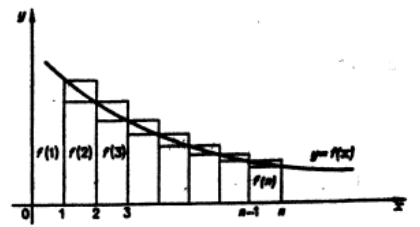
\includegraphics{leidn.png}
	$ c_1 \geq c_2 \geq \dots 0 , c_n \rightarrow 0 $\\
	Тогда $ 2(-1)^{n-1}c_n $-сходится\\ 
	\textbf{Секретное приложение}
	$ |\sum_{K \geq N}(-1)^{k-1}| \leq C_N $\\
	
	$ S_{2n} \uparrow,  S_{2n}+c_{2n+1} - c_{2n +2} > S_{2n+2}  \\
	S_{2n}$-ограничена сверху, $ S_{2n \leq c_1} \\
	S_{2n}= c_1 -  c_2 + c_3- c_{2n-2} + c_{2n-1}  - c_{2n}$ разность по парам 2n-2 и  2n-1  не больше нуля \\
	$ \exists \lim S_{2n} = S \\
	S_{2n+1}(\rightarrow S)=S_{2n}(\rightarrow S)+ c_{2n + 1}(\rightarrow 0) $\\
	\textbf{Очен грустный пример}\\
	$ (1)\sum \frac{(-1)^k}{\sqrt{k}+(-1)^k} \\
	(2)  \sum \frac{(-1)^k}{\sqrt{k}} \\
	\frac{(-1)^k}{\sqrt{k}+(-1)^k} - \frac{(-1)^k}{\sqrt{k}}=(-1)^k \frac{\sqrt{k} - \sqrt{k}+(-1)^k}{(\sqrt{k}+(-1)^k)\sqrt{k}}= -\frac{1}{(\sqrt{k}+(-1)^k \sqrt{k})} \sim_{k \rightarrow +\infty} - \frac{1}{k} \\$ -расходящийся \\
	$ (3) \sum \frac{(-1)^k}{\sqrt{k} + (-1)^k} - \frac{(-1)^k}{\sqrt{k}} = \sum \frac{-1}{(\sqrt{k})+(-1)^k \sqrt{k}} \\$
	Для знакоперемнных рядов  неверен признак сравнения \\
	$ a_n \sim b_n $и при этом  $\sum a_n$ -сходящ ,$ \sum b_n$-расходящ  \\ Это возможно. \\
	$ \sum \frac{(-1)^n}{\sqrt{n}}, \; a_n = \frac{(-1)^n}{\sqrt{n}} \\
	\sum (\frac{(-1)^n}{\sqrt{n}} +\frac{1}{n}), \; b_n = \frac{(-1)^n}{\sqrt{n}}+\frac{1}{n} == a_n + o(a+n)\\
	\int_{1}^{+ \infty} \frac{sin x}{\sqrt{x}} \; \int_1^{+\infty} \frac{\sin x}{\sqrt{x}} + \frac{\sin^2x }{x}   $- дает расхождение\\
	\section{Теорема(признак Абеля и Дирихле)}
	$ \boxed{D} A_n -\text{ограничена}: \exists C_A \forall b , |a_1 + a_2 + \dots a_n |\leq C_A \\
	b_n \text{- монотонна, ограничена } \exists c_b \forall n , |b_n|\leq C_n\\
	\text{Тогда} \sum a_n b_n \text{ -сходится}$\\
	\textbf{Доказательство}
	$ \boxed{D} \text{здесь тоже } \exists C_b, \forall n, | b_n| \leq C_b \\
	\sum_{k=1}^{n} a_kb_k = \underbrace{A_nb_b}_{\text{огр. бм}} + \underbrace{\sum_{k=1}^{n-1} (b_k - b_{k-1}) A_k}_{\sum_{k=1}^{n-1} |b_k - b_{k+1}| |A_k| \leq 	C_A \sum_{k=1}^{n-1} |b_k - b_{k+1}| = C_A |b_1 - b_n \leq C_A 2C_B| \text{такие суммы ограничены}} \\
	\Rightarrow \sum_{k=1}^{+\infty} |b_k - b_{k+1}||A_k|\text{-сходящ} \Rightarrow \sum_{k=1}^{+\infty} (b_k - b_{k+1})A_k\text{ - сходящийся]}$ \\
	\textbf{Пример}\\
	$ \sum_{n=1}^{+\infty} \frac{\sin n}{n^p} \\
	\text{?p - cx, ?p - абс. сх.} \\
	1. p=0 : \sum \sin n \text{-расходится,} \sin n \; not \rightarrow 0 \\
	p<0 \sum \frac{1}{n^p} \sin n  not \rightarrow 0 \\
	\text{нет схоидмости} \\
	2. p>1, \; |\frac{\sin n}{n^p}| \leq \frac{1}{n^p}, \;  \sum \frac{1}{n^p} \text{-сходящаяся} \\
	\sum \frac{\sin n}{n^p} \text{абс сх}\\
	3. p < p \leq 1, \text{сходятся по принципу Дирихле} \\
	D_n = \sin n \\
	b_N =\frac{1}{n^p} \longrightarrow 0 , \text{монотонна} \\
	\text{Проверим :} \exists C_A , \forall n : |\sin 1 +\sin 2 + \sin 3 + \dots + \sin n|\leq C_A\\$
	
	$ f(x+y) =f(x) f(y)\\
	\exp^{ix}= \cos x + i \sin x \; sinx = Im(\exp^{ix})\\
	\cos x = \frac{\exp^{ix} + \exp^{-ix}}{2}\\
	\sin x = \frac{\exp^{ix}-\exp^{-ix}}{2i} \\
	|\sin 1 + \dots+ \sin n | = |Im(E^I+ \dots \exp^{ni})| \leq |e^i+\dots + \exp^{ni}| = |e^i \frac{e^{ni} - 1 }{e^i -1}| = \underbrace{|e^i|}_{=1}|e^i| \frac{|e^{ni}-1|}{e^i -1} \leq \frac{2}{|e^i -1|} =: C_A \text{-используем геометрическую прогрессию}\\ 
	\sum |\frac{\sin n}{n^p}| \geq \sum \frac{\sin^2 n}{n^p}= \underbrace{\frac{1}{2}\sum \frac{1}{n^p}}_{+\infty} - \underbrace{\frac{1}{2}\sum\frac{\cos 2n}{n^p}}_{\text{кон. Ряд сходится по Дирихле}}$
	
	
	
=======
         \section{Сходимость  знакопеременных рядов}
         
         \subsection{Признак Лейбница}
        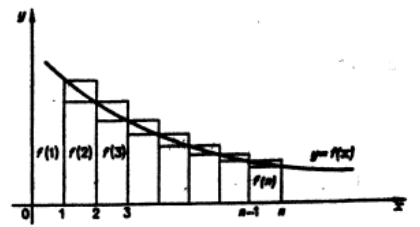
\includegraphics{leidn.png}
         $ c_1 \geq c_2 \geq \dots 0 , c_n \rightarrow 0 $\\
         Тогда $ 2(-1)^{n-1}c_n $-сходится\\ 
         \textbf{Секретное приложение}
         $ |\sum_{K \geq N}(-1)^{k-1}| \leq C_N $\\
         
         $ S_{2n} \uparrow,  S_{2n}+c_{2n+1} - c_{2n +2} > S_{2n+2}  \\
         S_{2n}$-ограничена сверху, $ S_{2n \leq c_1} \\
         S_{2n}= c_1 -  c_2 + c_3- c_{2n-2} + c_{2n-1}  - c_{2n}$ разность по парам 2n-2 и  2n-1  не больше нуля \\
         $ \exists \lim S_{2n} = S \\
         S_{2n+1}(\rightarrow S)=S_{2n}(\rightarrow S)+ c_{2n + 1}(\rightarrow 0) $\\
         \textbf{Очен грустный пример}\\
          $ (1)\sum \frac{(-1)^k}{\sqrt{k}+(-1)^k} \\
         (2)  \sum \frac{(-1)^k}{\sqrt{k}} \\
           \frac{(-1)^k}{\sqrt{k}+(-1)^k} - \frac{(-1)^k}{\sqrt{k}}=(-1)^k \frac{\sqrt{k} - \sqrt{k}+(-1)^k}{(\sqrt{k}+(-1)^k)\sqrt{k}}= -\frac{1}{(\sqrt{k}+(-1)^k \sqrt{k})} \sim_{k \rightarrow +\infty} - \frac{1}{k} \\$ -расходящийся \\
           $ (3) \sum \frac{(-1)^k}{\sqrt{k} + (-1)^k} - \frac{(-1)^k}{\sqrt{k}} = \sum \frac{-1}{(\sqrt{k})+(-1)^k \sqrt{k}} \\$
           Для знакоперемнных рядов  неверен признак сравнения \\
           $ a_n \sim b_n $и при этом  $\sum a_n$ -сходящ ,$ \sum b_n$-расходящ  \\ Это возможно. \\
           $ \sum \frac{(-1)^n}{\sqrt{n}}, \; a_n = \frac{(-1)^n}{\sqrt{n}} \\
           \sum (\frac{(-1)^n}{\sqrt{n}} +\frac{1}{n}), \; b_n = \frac{(-1)^n}{\sqrt{n}}+\frac{1}{n} == a_n + o(a+n)\\
           \int_{1}^{+ \infty} \frac{sin x}{\sqrt{x}} \; \int_1^{+\infty} \frac{\sin x}{\sqrt{x}} + \frac{\sin^2x }{x}   $- дает расхождение\\
           \section{Теорема(признак Абеля и Дирихле)}
           $ \boxed{D} A_n -\text{ограничена}: \exists C_A \forall b , |a_1 + a_2 + \dots a_n |\leq C_A \\
           b_n \text{- монотонна, ограничена } \exists c_b \forall n , |b_n|\leq C_n\\
           \text{Тогда} \sum a_n b_n \text{ -сходится}$\\
           \textbf{Доказательство}
          $ \boxed{D} \text{здесь тоже } \exists C_b, \forall n, | b_n| \leq C_b \\
          \sum_{k=1}^{n} a_kb_k = \underbrace{A_nb_b}_{\text{огр. бм}} + \underbrace{\sum_{k=1}^{n-1} (b_k - b_{k-1}) A_k}_{\sum_{k=1}^{n-1} |b_k - b_{k+1}| |A_k| \leq 	C_A \sum_{k=1}^{n-1} |b_k - b_{k+1}| = C_A |b_1 - b_n \leq C_A 2C_B| \text{такие суммы ограничены}} \\
          \Rightarrow \sum_{k=1}^{+\infty} |b_k - b_{k+1}||A_k|\text{-сходящ} \Rightarrow \sum_{k=1}^{+\infty} (b_k - b_{k+1})A_k\text{ - сходящийся]}$ \\
          \textbf{Пример}\\
          $ \sum_{n=1}^{+\infty} \frac{\sin n}{n^p} \\
          \text{?p - cx, ?p - абс. сх.} \\
          1. p=0 : \sum \sin n \text{-расходится,} \sin n \; not \rightarrow 0 \\
           p<0 \sum \frac{1}{n^p} \sin n  not \rightarrow 0 \\
           \text{нет схоидмости} \\
           2. p>1, \; |\frac{\sin n}{n^p}| \leq \frac{1}{n^p}, \;  \sum \frac{1}{n^p} \text{-сходящаяся} \\
           \sum \frac{\sin n}{n^p} \text{абс сх}\\
           3. p < p \leq 1, \text{сходятся по принципу Дирихле} \\
           D_n = \sin n \\
           b_N =\frac{1}{n^p} \longrightarrow 0 , \text{монотонна} \\
           \text{Проверим :} \exists C_A , \forall n : |\sin 1 +\sin 2 + \sin 3 + \dots + \sin n|\leq C_A\\$
           
           $ f(x+y) =f(x) f(y)\\
           \exp^{ix}= \cos x + i \sin x \; sinx = Im(\exp^{ix})\\
           \cos x = \frac{\exp^{ix} + \exp^{-ix}}{2}\\
            \sin x = \frac{\exp^{ix}-\exp^{-ix}}{2i} \\
            |\sin 1 + \dots+ \sin n | = |Im(E^I+ \dots \exp^{ni})| \leq |e^i+\dots + \exp^{ni}| = |e^i \frac{e^{ni} - 1 }{e^i -1}| = \underbrace{|e^i|}_{=1}|e^i| \frac{|e^{ni}-1|}{e^i -1} \leq \frac{2}{|e^i -1|} =: C_A \text{-используем геометрическую прогрессию}\\ 
            \sum |\frac{\sin n}{n^p}| \geq \sum \frac{\sin^2 n}{n^p}= \underbrace{\frac{1}{2}\sum \frac{1}{n^p}}_{+\infty} - \underbrace{\frac{1}{2}\sum\frac{\cos 2n}{n^p}}_{\text{кон. Ряд сходится по Дирихле}}$
        
       

>>>>>>> b05a3ab1132dcad2de454e7c5b07643779cd9508
	
	
\end{document}